\documentclass[twoside]{book}

% Packages required by doxygen
\usepackage{fixltx2e}
\usepackage{calc}
\usepackage{doxygen}
\usepackage[export]{adjustbox} % also loads graphicx
\usepackage{graphicx}
\usepackage[utf8]{inputenc}
\usepackage{makeidx}
\usepackage{multicol}
\usepackage{multirow}
\PassOptionsToPackage{warn}{textcomp}
\usepackage{textcomp}
\usepackage[nointegrals]{wasysym}
\usepackage[table]{xcolor}

% Font selection
\usepackage[T1]{fontenc}
\usepackage[scaled=.90]{helvet}
\usepackage{courier}
\usepackage{amssymb}
\usepackage{sectsty}
\renewcommand{\familydefault}{\sfdefault}
\allsectionsfont{%
  \fontseries{bc}\selectfont%
  \color{darkgray}%
}
\renewcommand{\DoxyLabelFont}{%
  \fontseries{bc}\selectfont%
  \color{darkgray}%
}
\newcommand{\+}{\discretionary{\mbox{\scriptsize$\hookleftarrow$}}{}{}}

% Page & text layout
\usepackage{geometry}
\geometry{%
  a4paper,%
  top=2.5cm,%
  bottom=2.5cm,%
  left=2.5cm,%
  right=2.5cm%
}
\tolerance=750
\hfuzz=15pt
\hbadness=750
\setlength{\emergencystretch}{15pt}
\setlength{\parindent}{0cm}
\setlength{\parskip}{3ex plus 2ex minus 2ex}
\makeatletter
\renewcommand{\paragraph}{%
  \@startsection{paragraph}{4}{0ex}{-1.0ex}{1.0ex}{%
    \normalfont\normalsize\bfseries\SS@parafont%
  }%
}
\renewcommand{\subparagraph}{%
  \@startsection{subparagraph}{5}{0ex}{-1.0ex}{1.0ex}{%
    \normalfont\normalsize\bfseries\SS@subparafont%
  }%
}
\makeatother

% Headers & footers
\usepackage{fancyhdr}
\pagestyle{fancyplain}
\fancyhead[LE]{\fancyplain{}{\bfseries\thepage}}
\fancyhead[CE]{\fancyplain{}{}}
\fancyhead[RE]{\fancyplain{}{\bfseries\leftmark}}
\fancyhead[LO]{\fancyplain{}{\bfseries\rightmark}}
\fancyhead[CO]{\fancyplain{}{}}
\fancyhead[RO]{\fancyplain{}{\bfseries\thepage}}
\fancyfoot[LE]{\fancyplain{}{}}
\fancyfoot[CE]{\fancyplain{}{}}
\fancyfoot[RE]{\fancyplain{}{\bfseries\scriptsize Generated by Doxygen }}
\fancyfoot[LO]{\fancyplain{}{\bfseries\scriptsize Generated by Doxygen }}
\fancyfoot[CO]{\fancyplain{}{}}
\fancyfoot[RO]{\fancyplain{}{}}
\renewcommand{\footrulewidth}{0.4pt}
\renewcommand{\chaptermark}[1]{%
  \markboth{#1}{}%
}
\renewcommand{\sectionmark}[1]{%
  \markright{\thesection\ #1}%
}

% Indices & bibliography
\usepackage{natbib}
\usepackage[titles]{tocloft}
\setcounter{tocdepth}{3}
\setcounter{secnumdepth}{5}
\makeindex

% Hyperlinks (required, but should be loaded last)
\usepackage{ifpdf}
\ifpdf
  \usepackage[pdftex,pagebackref=true]{hyperref}
\else
  \usepackage[ps2pdf,pagebackref=true]{hyperref}
\fi
\hypersetup{%
  colorlinks=true,%
  linkcolor=blue,%
  citecolor=blue,%
  unicode%
}

% Custom commands
\newcommand{\clearemptydoublepage}{%
  \newpage{\pagestyle{empty}\cleardoublepage}%
}

\usepackage{caption}
\captionsetup{labelsep=space,justification=centering,font={bf},singlelinecheck=off,skip=4pt,position=top}

%===== C O N T E N T S =====

\begin{document}

% Titlepage & ToC
\hypersetup{pageanchor=false,
             bookmarksnumbered=true,
             pdfencoding=unicode
            }
\pagenumbering{alph}
\begin{titlepage}
\vspace*{7cm}
\begin{center}%
{\Large Lib\+S\+S\+L\+AM\+: C++ library for object analysis in texture and depth images. }\\
\vspace*{1cm}
{\large Generated by Doxygen 1.8.13}\\
\end{center}
\end{titlepage}
\clearemptydoublepage
\pagenumbering{roman}
\tableofcontents
\clearemptydoublepage
\pagenumbering{arabic}
\hypersetup{pageanchor=true}

%--- Begin generated contents ---
\chapter{Class Index}
\section{Class List}
Here are the classes, structs, unions and interfaces with brief descriptions\+:\begin{DoxyCompactList}
\item\contentsline{section}{\hyperlink{classBaseSegmenter}{Base\+Segmenter} }{\pageref{classBaseSegmenter}}{}
\item\contentsline{section}{\hyperlink{classCloudViewer}{Cloud\+Viewer$<$ T $>$} }{\pageref{classCloudViewer}}{}
\item\contentsline{section}{\hyperlink{classDoN}{DoN} }{\pageref{classDoN}}{}
\item\contentsline{section}{\hyperlink{classEngine}{Engine} \\*An engine implementation to run object instance segmentation using maskrcnn-\/benchmark and O\+R\+B\+S\+L\+A\+M2 }{\pageref{classEngine}}{}
\item\contentsline{section}{\hyperlink{classGroundRemoval}{Ground\+Removal} \\*Ground Removal based on Ground Plane Fitting(\+G\+P\+F)  Fast Segmentation of 3D Point Clouds\+: A Paradigm on Li\+D\+AR Data for Autonomous Vehicle Applications (I\+C\+RA, 2017) }{\pageref{classGroundRemoval}}{}
\item\contentsline{section}{\hyperlink{classInstanceViewer}{Instance\+Viewer} }{\pageref{classInstanceViewer}}{}
\item\contentsline{section}{\hyperlink{structIntr}{Intr} }{\pageref{structIntr}}{}
\item\contentsline{section}{\hyperlink{classInventory}{Inventory} \\*An inventory of all detected and classified map objects }{\pageref{classInventory}}{}
\item\contentsline{section}{\hyperlink{classMaskRCNN}{Mask\+R\+C\+NN} \\*An interface between maskrcnn-\/benchmark in python and \hyperlink{classEngine}{Engine} in C++ }{\pageref{classMaskRCNN}}{}
\item\contentsline{section}{\hyperlink{structmodel__t}{model\+\_\+t} }{\pageref{structmodel__t}}{}
\item\contentsline{section}{\hyperlink{classObject}{Object} \\*A definition of an object in the inventory }{\pageref{classObject}}{}
\item\contentsline{section}{\hyperlink{classObjectDrawer}{Object\+Drawer} }{\pageref{classObjectDrawer}}{}
\item\contentsline{section}{\hyperlink{classObjectPoint}{Object\+Point} }{\pageref{classObjectPoint}}{}
\item\contentsline{section}{\hyperlink{classTSDF}{T\+S\+DF} \\*C\+U\+DA kernel function to integrate a \hyperlink{classTSDF}{T\+S\+DF} voxel volume given depth images }{\pageref{classTSDF}}{}
\item\contentsline{section}{\hyperlink{classTSDFfusion}{T\+S\+D\+Ffusion} \\*An interface between T\+S\+D\+F-\/fusion-\/python in python and \hyperlink{classEngine}{Engine} in C++ }{\pageref{classTSDFfusion}}{}
\end{DoxyCompactList}

\chapter{Class Documentation}
\hypertarget{classBaseSegmenter}{}\section{Base\+Segmenter Class Reference}
\label{classBaseSegmenter}\index{Base\+Segmenter@{Base\+Segmenter}}
\subsection*{Public Member Functions}
\begin{DoxyCompactItemize}
\item 
\mbox{\Hypertarget{classBaseSegmenter_adbb7ea25f30ec103541b24118fc36f36}\label{classBaseSegmenter_adbb7ea25f30ec103541b24118fc36f36}} 
virtual void \hyperlink{classBaseSegmenter_adbb7ea25f30ec103541b24118fc36f36}{segment} (const pcl\+::\+Point\+Cloud$<$ Point\+Type $>$ \&cloud\+\_\+in, std\+::vector$<$ pcl\+::\+Point\+Cloud$<$ Point\+Type $>$\+::Ptr $>$ \&cloud\+\_\+clusters)=0
\begin{DoxyCompactList}\small\item\em Segment the point cloud. \end{DoxyCompactList}\item 
\mbox{\Hypertarget{classBaseSegmenter_afd4e2673d8ce2d6ab36ec09dd34aa766}\label{classBaseSegmenter_afd4e2673d8ce2d6ab36ec09dd34aa766}} 
virtual std\+::string {\bfseries name} () const =0
\end{DoxyCompactItemize}


The documentation for this class was generated from the following file\+:\begin{DoxyCompactItemize}
\item 
/home/mrt/\+Dev/maskrcnn\+\_\+slam\+\_\+b/include/base\+\_\+segmenter.\+hpp\end{DoxyCompactItemize}

\hypertarget{classCloudViewer}{}\section{Cloud\+Viewer$<$ T $>$ Class Template Reference}
\label{classCloudViewer}\index{Cloud\+Viewer$<$ T $>$@{Cloud\+Viewer$<$ T $>$}}
\subsection*{Public Member Functions}
\begin{DoxyCompactItemize}
\item 
\mbox{\Hypertarget{classCloudViewer_aa91e5e3696d55cbe76e28f112baf4725}\label{classCloudViewer_aa91e5e3696d55cbe76e28f112baf4725}} 
{\bfseries Cloud\+Viewer} (typename pcl\+::\+Point\+Cloud$<$ T $>$\+::Ptr Cloud, std\+::vector$<$ pcl\+::\+Point\+Indices $>$ Clusters)
\item 
\mbox{\Hypertarget{classCloudViewer_a415fb5c3c3f39d3c6b73d9e9fb27290f}\label{classCloudViewer_a415fb5c3c3f39d3c6b73d9e9fb27290f}} 
{\bfseries Cloud\+Viewer} (typename pcl\+::\+Point\+Cloud$<$ T $>$\+::Ptr Cloud)
\item 
\mbox{\Hypertarget{classCloudViewer_a5437cd2efaf18711dd646db18e01934e}\label{classCloudViewer_a5437cd2efaf18711dd646db18e01934e}} 
void {\bfseries Run} ()
\end{DoxyCompactItemize}


The documentation for this class was generated from the following file\+:\begin{DoxyCompactItemize}
\item 
/home/mrt/\+Dev/maskrcnn\+\_\+slam\+\_\+b/include/Cloud\+Viewer.\+hpp\end{DoxyCompactItemize}

\hypertarget{classDoN}{}\section{DoN Class Reference}
\label{classDoN}\index{DoN@{DoN}}
\subsection*{Public Member Functions}
\begin{DoxyCompactItemize}
\item 
\mbox{\Hypertarget{classDoN_a65b2219f2c0aa71596cf50608b1bb827}\label{classDoN_a65b2219f2c0aa71596cf50608b1bb827}} 
\hyperlink{classDoN_a65b2219f2c0aa71596cf50608b1bb827}{DoN} ()
\begin{DoxyCompactList}\small\item\em Default constructor. \end{DoxyCompactList}\item 
\mbox{\Hypertarget{classDoN_a9c5679670e784bddfca231c63122bce7}\label{classDoN_a9c5679670e784bddfca231c63122bce7}} 
\hyperlink{classDoN_a9c5679670e784bddfca231c63122bce7}{DoN} (double scale1, double scale2, double threshold, double segradius)
\begin{DoxyCompactList}\small\item\em Constructor with inputs. \end{DoxyCompactList}\item 
\mbox{\Hypertarget{classDoN_a8583a85e01c683f503decb1a8a757682}\label{classDoN_a8583a85e01c683f503decb1a8a757682}} 
\hyperlink{classDoN_a8583a85e01c683f503decb1a8a757682}{DoN} (double scale1, double scale2, double threshold, double segradius, cv\+::\+Mat K, int im\+Width, int im\+Height, int)
\begin{DoxyCompactList}\small\item\em Constructor with more image inputs. \end{DoxyCompactList}\item 
\mbox{\Hypertarget{classDoN_a4544ca7d9278dffa111202464c005aad}\label{classDoN_a4544ca7d9278dffa111202464c005aad}} 
\hyperlink{classDoN_a4544ca7d9278dffa111202464c005aad}{$\sim$\+DoN} ()
\begin{DoxyCompactList}\small\item\em Default destructor. \end{DoxyCompactList}\item 
std\+::map$<$ int, std\+::vector$<$ cv\+::\+Point $>$ $>$ \hyperlink{classDoN_ae1e63b9178dad44c2ced58bd571253cd}{extract} (cv\+::\+Mat \&im\+R\+GB, cv\+::\+Mat \&imD)
\begin{DoxyCompactList}\small\item\em The main function to cluster the depth data. \end{DoxyCompactList}\item 
void \hyperlink{classDoN_ad64458603d62f8a04298520cb747b90e}{extract} (pcl\+::\+Point\+Cloud$<$ pcl\+::\+Point\+X\+Y\+ZI $>$\+::Ptr cloud)
\item 
\mbox{\Hypertarget{classDoN_aa0cffa1275c78488726dab2635265c05}\label{classDoN_aa0cffa1275c78488726dab2635265c05}} 
std\+::map$<$ int, std\+::vector$<$ cv\+::\+Point $>$ $>$ \hyperlink{classDoN_aa0cffa1275c78488726dab2635265c05}{Get\+Clusters} ()
\begin{DoxyCompactList}\small\item\em Obselete function\+: returns a vector of clusters in image coordinates. \end{DoxyCompactList}\item 
\mbox{\Hypertarget{classDoN_a32f62241f82a021cbf44cefaee8f800d}\label{classDoN_a32f62241f82a021cbf44cefaee8f800d}} 
void \hyperlink{classDoN_a32f62241f82a021cbf44cefaee8f800d}{show2d} (cv\+::\+Mat \&im\+R\+GB)
\begin{DoxyCompactList}\small\item\em 2D visualisation function, which requires and input image to display clusters on. \end{DoxyCompactList}\item 
\mbox{\Hypertarget{classDoN_a1d5a069af68c05bc2b525d42b8b9e94a}\label{classDoN_a1d5a069af68c05bc2b525d42b8b9e94a}} 
void \hyperlink{classDoN_a1d5a069af68c05bc2b525d42b8b9e94a}{show3d} ()
\begin{DoxyCompactList}\small\item\em 3D visualisation function. \end{DoxyCompactList}\item 
\mbox{\Hypertarget{classDoN_a704e464039afd6d573c11ca57fc800be}\label{classDoN_a704e464039afd6d573c11ca57fc800be}} 
pcl\+::\+Point\+Cloud$<$ pcl\+::\+Point\+Normal $>$\+::Ptr {\bfseries Get\+Don\+Cloud} ()
\item 
\mbox{\Hypertarget{classDoN_a79aa2357440c81f36cf99902cf24e47e}\label{classDoN_a79aa2357440c81f36cf99902cf24e47e}} 
std\+::vector$<$ pcl\+::\+Point\+Indices $>$ {\bfseries Get\+Clusters\+Indices} ()
\end{DoxyCompactItemize}


\subsection{Member Function Documentation}
\mbox{\Hypertarget{classDoN_ae1e63b9178dad44c2ced58bd571253cd}\label{classDoN_ae1e63b9178dad44c2ced58bd571253cd}} 
\index{DoN@{DoN}!extract@{extract}}
\index{extract@{extract}!DoN@{DoN}}
\subsubsection{\texorpdfstring{extract()}{extract()}\hspace{0.1cm}{\footnotesize\ttfamily [1/2]}}
{\footnotesize\ttfamily std\+::map$<$ int, std\+::vector$<$ cv\+::\+Point $>$ $>$ Do\+N\+::extract (\begin{DoxyParamCaption}\item[{cv\+::\+Mat \&}]{im\+R\+GB,  }\item[{cv\+::\+Mat \&}]{imD }\end{DoxyParamCaption})}



The main function to cluster the depth data. 

N\+O\+TE\+: setting viewpoint is very important, so that we can ensure normals are all pointed in the same direction!\mbox{\Hypertarget{classDoN_ad64458603d62f8a04298520cb747b90e}\label{classDoN_ad64458603d62f8a04298520cb747b90e}} 
\index{DoN@{DoN}!extract@{extract}}
\index{extract@{extract}!DoN@{DoN}}
\subsubsection{\texorpdfstring{extract()}{extract()}\hspace{0.1cm}{\footnotesize\ttfamily [2/2]}}
{\footnotesize\ttfamily void Do\+N\+::extract (\begin{DoxyParamCaption}\item[{pcl\+::\+Point\+Cloud$<$ pcl\+::\+Point\+X\+Y\+ZI $>$\+::Ptr}]{cloud }\end{DoxyParamCaption})}

N\+O\+TE\+: setting viewpoint is very important, so that we can ensure normals are all pointed in the same direction!

The documentation for this class was generated from the following files\+:\begin{DoxyCompactItemize}
\item 
/home/mrt/\+Dev/maskrcnn\+\_\+slam\+\_\+b/include/Do\+N.\+hpp\item 
/home/mrt/\+Dev/maskrcnn\+\_\+slam\+\_\+b/src/Do\+N.\+cpp\end{DoxyCompactItemize}

\hypertarget{classEngine}{}\section{Engine Class Reference}
\label{classEngine}\index{Engine@{Engine}}


An engine implementation to run object instance segmentation using maskrcnn-\/benchmark and O\+R\+B\+S\+L\+A\+M2.  




{\ttfamily \#include $<$Engine.\+hpp$>$}



Collaboration diagram for Engine\+:\nopagebreak
\begin{figure}[H]
\begin{center}
\leavevmode
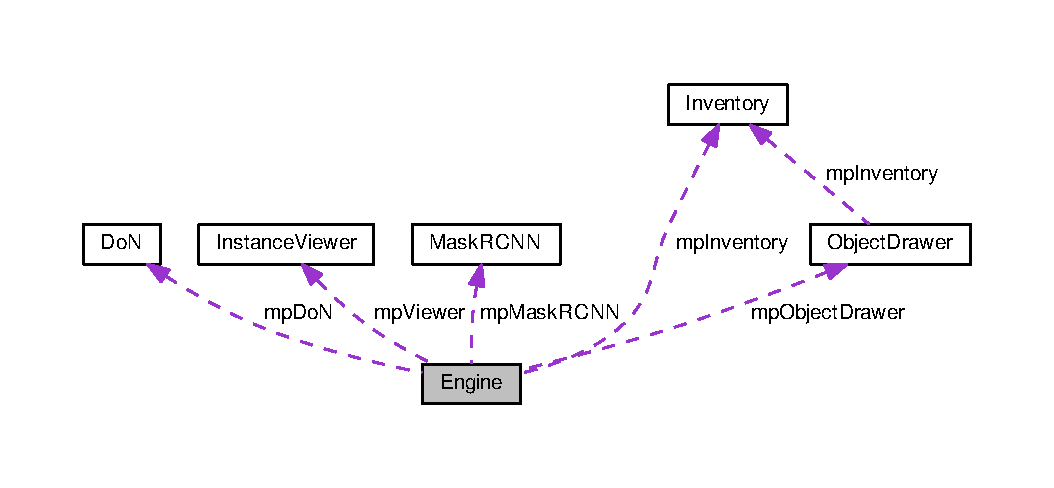
\includegraphics[width=350pt]{classEngine__coll__graph}
\end{center}
\end{figure}
\subsection*{Public Member Functions}
\begin{DoxyCompactItemize}
\item 
\hyperlink{classEngine_ab3818182cd3d2b3a788ac04d743cf6f4}{Engine} (std\+::unordered\+\_\+map$<$ int, std\+::string $>$ categories, std\+::string)
\item 
\hyperlink{classEngine_a8ef7030a089ecb30bbfcb9e43094717a}{$\sim$\+Engine} ()
\item 
void \hyperlink{classEngine_a0e1fdb5ff8c992b1795eff03e2551708}{Run} (cv\+::\+Mat im\+R\+GB, cv\+::\+Mat imD, Key\+Frame $\ast$KF)
\item 
\hyperlink{classObject}{Object} $\ast$ \hyperlink{classEngine_ad6d6151754fc9b77c75ce041f4653007}{Track\+Object\+Points} (Contour mask\+Contour, const std\+::string label, double score, cv\+::\+Mat im\+Depth)
\item 
\hyperlink{classObject}{Object} $\ast$ \hyperlink{classEngine_a76d6ccc8e7dd30849fbcb039cd8cf5a6}{Track\+Object\+Contours} (Contour mask\+Contour, const std\+::string label, double score, cv\+::\+Mat im\+Depth)
\item 
cv\+::\+Point \hyperlink{classEngine_ab7feb6f45507d808379e9c4ba6cae90b}{Project\+Into\+Current\+KF} (\hyperlink{classObjectPoint}{Object\+Point} $\ast$MP)
\item 
cv\+::\+Mat \hyperlink{classEngine_a381792d9c8cf59c365aa9ef5ff1841fb}{Compute\+Fundamental} (Key\+Frame $\ast$K\+F1, Key\+Frame $\ast$K\+F2)
\item 
cv\+::\+Mat \hyperlink{classEngine_ade7b2b448a71642155d74932139c26d7}{Get\+Skew\+Symmetric\+Matrix} (const cv\+::\+Mat \&v)
\item 
float \hyperlink{classEngine_a21c2286837892a045674c6e9c2aaa0b8}{shortest\+\_\+distance} (float u, float v, float a, float b, float c)
\item 
void \hyperlink{classEngine_a45c5502ceecdd852f9417ed0d7c73648}{display} (\hyperlink{classObject}{Object} $\ast$O, cv\+::\+Mat im\+R\+GB, Contour mask\+Contour, cv\+::\+Rect bbox, std\+::vector$<$ cv\+::\+Vec4i $>$ hierarchy, cv\+::\+Scalar color)
\item 
\mbox{\Hypertarget{classEngine_adbb2bcd0cf0e2f084226f38477a871a9}\label{classEngine_adbb2bcd0cf0e2f084226f38477a871a9}} 
bool {\bfseries Is\+In\+Current\+KF} (float range, cv\+::\+Point cvpoint, int margin)
\end{DoxyCompactItemize}
\subsection*{Protected Types}
\begin{DoxyCompactItemize}
\item 
\mbox{\Hypertarget{classEngine_aabf30721fe5b9d5a0596aceddf4fc8ad}\label{classEngine_aabf30721fe5b9d5a0596aceddf4fc8ad}} 
typedef std\+::chrono\+::monotonic\+\_\+clock\+::time\+\_\+point {\bfseries timer}
\end{DoxyCompactItemize}
\subsection*{Protected Member Functions}
\begin{DoxyCompactItemize}
\item 
\mbox{\Hypertarget{classEngine_a862870af01354ec1327bae82074e836f}\label{classEngine_a862870af01354ec1327bae82074e836f}} 
void {\bfseries tick} ()
\item 
\mbox{\Hypertarget{classEngine_a09c7704a2bef626ce6c80e504a178bf9}\label{classEngine_a09c7704a2bef626ce6c80e504a178bf9}} 
double {\bfseries tock} ()
\item 
\mbox{\Hypertarget{classEngine_a8236c8dbd88d7398fa135e9d660217a2}\label{classEngine_a8236c8dbd88d7398fa135e9d660217a2}} 
{\footnotesize template$<$class T $>$ }\\T {\bfseries tick} ()
\item 
\mbox{\Hypertarget{classEngine_a2823156001f3e2bbdbcbdb4d29322272}\label{classEngine_a2823156001f3e2bbdbcbdb4d29322272}} 
{\footnotesize template$<$class T $>$ }\\double {\bfseries tock} (T t1)
\end{DoxyCompactItemize}
\subsection*{Protected Attributes}
\begin{DoxyCompactItemize}
\item 
\mbox{\Hypertarget{classEngine_a32fcfaf08165cdfc81d39e8dc8d71e6f}\label{classEngine_a32fcfaf08165cdfc81d39e8dc8d71e6f}} 
int {\bfseries m\+Sensor}
\item 
\mbox{\Hypertarget{classEngine_a7c6071c21007bd703040b035f4262da8}\label{classEngine_a7c6071c21007bd703040b035f4262da8}} 
float \hyperlink{classEngine_a7c6071c21007bd703040b035f4262da8}{mn\+Min\+Depth}
\begin{DoxyCompactList}\small\item\em Minimum perceived depth. \end{DoxyCompactList}\item 
\mbox{\Hypertarget{classEngine_a639e031e36ea33902eee3bf4f2c4600f}\label{classEngine_a639e031e36ea33902eee3bf4f2c4600f}} 
float \hyperlink{classEngine_a639e031e36ea33902eee3bf4f2c4600f}{mn\+Max\+Depth}
\begin{DoxyCompactList}\small\item\em Maximum perceived depth. \end{DoxyCompactList}\item 
\mbox{\Hypertarget{classEngine_a1b1b9bc3ce76e792ae67818a36bd01bd}\label{classEngine_a1b1b9bc3ce76e792ae67818a36bd01bd}} 
float \hyperlink{classEngine_a1b1b9bc3ce76e792ae67818a36bd01bd}{mn\+Dist}
\begin{DoxyCompactList}\small\item\em Threshold for point-\/to-\/polygon test. \end{DoxyCompactList}\item 
\mbox{\Hypertarget{classEngine_a35ddf071177f32315a8e5d534005b907}\label{classEngine_a35ddf071177f32315a8e5d534005b907}} 
float {\bfseries m\+Min\+Area}
\item 
\mbox{\Hypertarget{classEngine_a470e699fd14551987d1a14e8227462e2}\label{classEngine_a470e699fd14551987d1a14e8227462e2}} 
float {\bfseries m\+Max\+Area}
\item 
\mbox{\Hypertarget{classEngine_a94359672a475890b50acc354ef174417}\label{classEngine_a94359672a475890b50acc354ef174417}} 
float {\bfseries m\+Overlap}
\item 
\mbox{\Hypertarget{classEngine_a30a62cf18615cc5bddad798ffcc3e12a}\label{classEngine_a30a62cf18615cc5bddad798ffcc3e12a}} 
int {\bfseries m\+Min\+Point\+Count}
\item 
\mbox{\Hypertarget{classEngine_a30d46eb3926affc633a70e49069d111f}\label{classEngine_a30d46eb3926affc633a70e49069d111f}} 
float {\bfseries m\+Prob\+Thd}
\item 
\mbox{\Hypertarget{classEngine_a915a94d5480ef2870041b5ff5f82ea0e}\label{classEngine_a915a94d5480ef2870041b5ff5f82ea0e}} 
float {\bfseries m\+Res}
\item 
cv\+::\+Mat \hyperlink{classEngine_a39ebc85b2ec8b863a9a525a4fa4689aa}{K}
\begin{DoxyCompactList}\small\item\em Camera intrinsic parameters (T\+UM) \end{DoxyCompactList}\item 
\mbox{\Hypertarget{classEngine_a9bddf06ba7cf3410c6b49fc865f1201c}\label{classEngine_a9bddf06ba7cf3410c6b49fc865f1201c}} 
cv\+::\+Mat \hyperlink{classEngine_a9bddf06ba7cf3410c6b49fc865f1201c}{Dist\+Coef}
\begin{DoxyCompactList}\small\item\em Camera lense distortion parameters. \end{DoxyCompactList}\item 
\mbox{\Hypertarget{classEngine_a08215fba7b1d3b3e9347d40590b5b54b}\label{classEngine_a08215fba7b1d3b3e9347d40590b5b54b}} 
int {\bfseries m\+Width}
\item 
\mbox{\Hypertarget{classEngine_a76d3938e3e8b6325ebae501696631d06}\label{classEngine_a76d3938e3e8b6325ebae501696631d06}} 
int {\bfseries m\+Height}
\item 
\mbox{\Hypertarget{classEngine_ab05ac5f81adf467caf2d9fb49113d704}\label{classEngine_ab05ac5f81adf467caf2d9fb49113d704}} 
Key\+Frame $\ast$ {\bfseries mp\+Current\+KF}
\item 
\mbox{\Hypertarget{classEngine_ac4c620f056b94de7faf0dfc13010d189}\label{classEngine_ac4c620f056b94de7faf0dfc13010d189}} 
\hyperlink{classMaskRCNN}{Mask\+R\+C\+NN} $\ast$ \hyperlink{classEngine_ac4c620f056b94de7faf0dfc13010d189}{mp\+Mask\+R\+C\+NN}
\begin{DoxyCompactList}\small\item\em A pointer to maskrcnn object. \end{DoxyCompactList}\item 
\mbox{\Hypertarget{classEngine_a94c02a735a6d30121bff171cbf96e7e1}\label{classEngine_a94c02a735a6d30121bff171cbf96e7e1}} 
\hyperlink{classDoN}{DoN} $\ast$ \hyperlink{classEngine_a94c02a735a6d30121bff171cbf96e7e1}{mp\+DoN}
\begin{DoxyCompactList}\small\item\em A pointer to \hyperlink{classDoN}{DoN} object. \end{DoxyCompactList}\item 
\mbox{\Hypertarget{classEngine_a1f29333d26ca0799ece0aad9a121108d}\label{classEngine_a1f29333d26ca0799ece0aad9a121108d}} 
std\+::unordered\+\_\+map$<$ int, std\+::string $>$ \hyperlink{classEngine_a1f29333d26ca0799ece0aad9a121108d}{mm\+Categories}
\begin{DoxyCompactList}\small\item\em Labelled object categories. \end{DoxyCompactList}\item 
\mbox{\Hypertarget{classEngine_ab1a7b510fc78ce3e41afcce0492c8065}\label{classEngine_ab1a7b510fc78ce3e41afcce0492c8065}} 
\hyperlink{classInventory}{Inventory} $\ast$ \hyperlink{classEngine_ab1a7b510fc78ce3e41afcce0492c8065}{mp\+Inventory}
\begin{DoxyCompactList}\small\item\em A pointer to \hyperlink{classInventory}{Inventory}. \end{DoxyCompactList}\item 
\mbox{\Hypertarget{classEngine_a344b73834a2105c834df216935af06e9}\label{classEngine_a344b73834a2105c834df216935af06e9}} 
\hyperlink{classInstanceViewer}{Instance\+Viewer} $\ast$ \hyperlink{classEngine_a344b73834a2105c834df216935af06e9}{mp\+Viewer}
\begin{DoxyCompactList}\small\item\em A pointer to \hyperlink{classObject}{Object} viewer. \end{DoxyCompactList}\item 
\mbox{\Hypertarget{classEngine_ae0baa7948abc47c2a198bd70eacea10c}\label{classEngine_ae0baa7948abc47c2a198bd70eacea10c}} 
\hyperlink{classObjectDrawer}{Object\+Drawer} $\ast$ \hyperlink{classEngine_ae0baa7948abc47c2a198bd70eacea10c}{mp\+Object\+Drawer}
\begin{DoxyCompactList}\small\item\em A pointer to \hyperlink{classObject}{Object} drawer. \end{DoxyCompactList}\item 
\mbox{\Hypertarget{classEngine_ac18e97590b413588ec2e0d91b06f9f8c}\label{classEngine_ac18e97590b413588ec2e0d91b06f9f8c}} 
std\+::thread $\ast$ \hyperlink{classEngine_ac18e97590b413588ec2e0d91b06f9f8c}{mpt\+Viewer}
\begin{DoxyCompactList}\small\item\em A pointer to \hyperlink{classObject}{Object} viewer thread. \end{DoxyCompactList}\item 
\mbox{\Hypertarget{classEngine_ad6aea740916785e00aa7f0bc7e73dbab}\label{classEngine_ad6aea740916785e00aa7f0bc7e73dbab}} 
timer {\bfseries mtimer}
\item 
\mbox{\Hypertarget{classEngine_ae9d68b104f8ed664e4dfb058dd360e7b}\label{classEngine_ae9d68b104f8ed664e4dfb058dd360e7b}} 
bool {\bfseries time\+Is\+Ticked} = false
\end{DoxyCompactItemize}


\subsection{Detailed Description}
An engine implementation to run object instance segmentation using maskrcnn-\/benchmark and O\+R\+B\+S\+L\+A\+M2. 

\begin{DoxyAuthor}{Author}
Tariq Abuhashim 
\end{DoxyAuthor}
\begin{DoxyDate}{Date}
August 2019 
\end{DoxyDate}


\subsection{Constructor \& Destructor Documentation}
\mbox{\Hypertarget{classEngine_ab3818182cd3d2b3a788ac04d743cf6f4}\label{classEngine_ab3818182cd3d2b3a788ac04d743cf6f4}} 
\index{Engine@{Engine}!Engine@{Engine}}
\index{Engine@{Engine}!Engine@{Engine}}
\subsubsection{\texorpdfstring{Engine()}{Engine()}}
{\footnotesize\ttfamily Engine\+::\+Engine (\begin{DoxyParamCaption}\item[{std\+::unordered\+\_\+map$<$ int, std\+::string $>$}]{categories,  }\item[{std\+::string}]{ }\end{DoxyParamCaption})}

Constructor, Initialises Mask-\/\+R\+C\+NN. 
\begin{DoxyParams}{Parameters}
{\em categories} & a map of integers and object class labels of type unordered\+\_\+map$<$int,string$>$ \\
\hline
\end{DoxyParams}
\mbox{\Hypertarget{classEngine_a8ef7030a089ecb30bbfcb9e43094717a}\label{classEngine_a8ef7030a089ecb30bbfcb9e43094717a}} 
\index{Engine@{Engine}!````~Engine@{$\sim$\+Engine}}
\index{````~Engine@{$\sim$\+Engine}!Engine@{Engine}}
\subsubsection{\texorpdfstring{$\sim$\+Engine()}{~Engine()}}
{\footnotesize\ttfamily Engine\+::$\sim$\+Engine (\begin{DoxyParamCaption}{ }\end{DoxyParamCaption})}

Default destructor, Deletes Mask-\/\+R\+C\+NN. 

\subsection{Member Function Documentation}
\mbox{\Hypertarget{classEngine_a381792d9c8cf59c365aa9ef5ff1841fb}\label{classEngine_a381792d9c8cf59c365aa9ef5ff1841fb}} 
\index{Engine@{Engine}!Compute\+Fundamental@{Compute\+Fundamental}}
\index{Compute\+Fundamental@{Compute\+Fundamental}!Engine@{Engine}}
\subsubsection{\texorpdfstring{Compute\+Fundamental()}{ComputeFundamental()}}
{\footnotesize\ttfamily cv\+::\+Mat Engine\+::\+Compute\+Fundamental (\begin{DoxyParamCaption}\item[{Key\+Frame $\ast$}]{K\+F1,  }\item[{Key\+Frame $\ast$}]{K\+F2 }\end{DoxyParamCaption})}

Computes the fundamental matrix between two O\+R\+B\+S\+L\+A\+M2 Key\+Frames (projects a 2D point in K\+F1 to a line in K\+F2) 
\begin{DoxyParams}{Parameters}
{\em K\+F1} & a pointer to the first (reference) Key\+Frame. \\
\hline
{\em K\+F2} & a pointer to the second Key\+Frame. \\
\hline
\end{DoxyParams}
\mbox{\Hypertarget{classEngine_a45c5502ceecdd852f9417ed0d7c73648}\label{classEngine_a45c5502ceecdd852f9417ed0d7c73648}} 
\index{Engine@{Engine}!display@{display}}
\index{display@{display}!Engine@{Engine}}
\subsubsection{\texorpdfstring{display()}{display()}}
{\footnotesize\ttfamily void Engine\+::display (\begin{DoxyParamCaption}\item[{\hyperlink{classObject}{Object} $\ast$}]{O,  }\item[{cv\+::\+Mat}]{im\+R\+GB,  }\item[{Contour}]{mask\+Contour,  }\item[{cv\+::\+Rect}]{bbox,  }\item[{std\+::vector$<$ cv\+::\+Vec4i $>$}]{hierarchy,  }\item[{cv\+::\+Scalar}]{color }\end{DoxyParamCaption})}

Displays object measurements in 2D on the image. This includes object contours and 3D points projections in the current Key\+Frame 
\begin{DoxyParams}{Parameters}
{\em O} & a pointer to the object \\
\hline
{\em im\+R\+GB} & the current R\+GB image \\
\hline
{\em KF} & the current Key\+Frame \\
\hline
{\em mask\+Contour} & a vector of visible object contours in the current Key\+Frame \\
\hline
{\em bbox} & an Open\+CV rectangular coordinates of the current object bounding box \\
\hline
{\em hierarchy} & Open\+CV contours hierarchy \\
\hline
{\em color} & display color for both, contours and 2D Object\+Points \\
\hline
\end{DoxyParams}
\mbox{\Hypertarget{classEngine_ade7b2b448a71642155d74932139c26d7}\label{classEngine_ade7b2b448a71642155d74932139c26d7}} 
\index{Engine@{Engine}!Get\+Skew\+Symmetric\+Matrix@{Get\+Skew\+Symmetric\+Matrix}}
\index{Get\+Skew\+Symmetric\+Matrix@{Get\+Skew\+Symmetric\+Matrix}!Engine@{Engine}}
\subsubsection{\texorpdfstring{Get\+Skew\+Symmetric\+Matrix()}{GetSkewSymmetricMatrix()}}
{\footnotesize\ttfamily cv\+::\+Mat Engine\+::\+Get\+Skew\+Symmetric\+Matrix (\begin{DoxyParamCaption}\item[{const cv\+::\+Mat \&}]{v }\end{DoxyParamCaption})}

Generates skew-\/symmetric square matrix (3x3) from an input vector 
\begin{DoxyParams}{Parameters}
{\em v} & input vector with dimensions (3x1) \\
\hline
\end{DoxyParams}
\mbox{\Hypertarget{classEngine_ab7feb6f45507d808379e9c4ba6cae90b}\label{classEngine_ab7feb6f45507d808379e9c4ba6cae90b}} 
\index{Engine@{Engine}!Project\+Into\+Current\+KF@{Project\+Into\+Current\+KF}}
\index{Project\+Into\+Current\+KF@{Project\+Into\+Current\+KF}!Engine@{Engine}}
\subsubsection{\texorpdfstring{Project\+Into\+Current\+K\+F()}{ProjectIntoCurrentKF()}}
{\footnotesize\ttfamily cv\+::\+Point Engine\+::\+Project\+Into\+Current\+KF (\begin{DoxyParamCaption}\item[{\hyperlink{classObjectPoint}{Object\+Point} $\ast$}]{MP }\end{DoxyParamCaption})}

Projects a map point from 3D into 2D image frame 
\begin{DoxyParams}{Parameters}
{\em MP} & a pointer to the current \hyperlink{classObjectPoint}{Object\+Point}. \\
\hline
\end{DoxyParams}
\mbox{\Hypertarget{classEngine_a0e1fdb5ff8c992b1795eff03e2551708}\label{classEngine_a0e1fdb5ff8c992b1795eff03e2551708}} 
\index{Engine@{Engine}!Run@{Run}}
\index{Run@{Run}!Engine@{Engine}}
\subsubsection{\texorpdfstring{Run()}{Run()}}
{\footnotesize\ttfamily void Engine\+::\+Run (\begin{DoxyParamCaption}\item[{cv\+::\+Mat}]{im\+R\+GB,  }\item[{cv\+::\+Mat}]{imD,  }\item[{Key\+Frame $\ast$}]{KF }\end{DoxyParamCaption})}

Main function to run the object instance segmentation process 
\begin{DoxyParams}{Parameters}
{\em im\+R\+GB} & is the current Key\+Frame R\+GB image \\
\hline
{\em imD} & is the current Key\+Frame depth image \\
\hline
{\em KF} & pointer to the current Key\+Frame \\
\hline
\end{DoxyParams}
\mbox{\Hypertarget{classEngine_a21c2286837892a045674c6e9c2aaa0b8}\label{classEngine_a21c2286837892a045674c6e9c2aaa0b8}} 
\index{Engine@{Engine}!shortest\+\_\+distance@{shortest\+\_\+distance}}
\index{shortest\+\_\+distance@{shortest\+\_\+distance}!Engine@{Engine}}
\subsubsection{\texorpdfstring{shortest\+\_\+distance()}{shortest\_distance()}}
{\footnotesize\ttfamily float Engine\+::shortest\+\_\+distance (\begin{DoxyParamCaption}\item[{float}]{u,  }\item[{float}]{v,  }\item[{float}]{a,  }\item[{float}]{b,  }\item[{float}]{c }\end{DoxyParamCaption})}

Calculates the shorted distance between a 2D point and a 2D line ( a$\ast$x + b$\ast$y + c = 0 ) 
\begin{DoxyParams}{Parameters}
{\em u} & horizontal coordinate of the 2D point in the image \\
\hline
{\em v} & vertical coordinate of the 2D point in the image \\
\hline
{\em a} & first line coefficient (first component of the normal vector to the line) \\
\hline
{\em b} & second line coefficient (second component of the normal vector to the line) \\
\hline
{\em c} & third line coefficient \\
\hline
\end{DoxyParams}
\mbox{\Hypertarget{classEngine_a76d6ccc8e7dd30849fbcb039cd8cf5a6}\label{classEngine_a76d6ccc8e7dd30849fbcb039cd8cf5a6}} 
\index{Engine@{Engine}!Track\+Object\+Contours@{Track\+Object\+Contours}}
\index{Track\+Object\+Contours@{Track\+Object\+Contours}!Engine@{Engine}}
\subsubsection{\texorpdfstring{Track\+Object\+Contours()}{TrackObjectContours()}}
{\footnotesize\ttfamily \hyperlink{classObject}{Object} $\ast$ Engine\+::\+Track\+Object\+Contours (\begin{DoxyParamCaption}\item[{Contour}]{mask\+Contour,  }\item[{const std\+::string}]{label,  }\item[{double}]{score,  }\item[{cv\+::\+Mat}]{im\+Depth }\end{DoxyParamCaption})}

Implements object instance tracking in images by tracking its contours and using epipolar geometry 
\begin{DoxyParams}{Parameters}
{\em mask\+Contour} & a vector of object contours extracted using Open\+CV. \\
\hline
{\em label} & the classification label of the detection object using \hyperlink{classMaskRCNN}{Mask\+R\+C\+NN}. \\
\hline
{\em score} & the classification score of the detection object using \hyperlink{classMaskRCNN}{Mask\+R\+C\+NN}. \\
\hline
{\em im\+Depth} & the current depth image. \\
\hline
\end{DoxyParams}
\mbox{\Hypertarget{classEngine_ad6d6151754fc9b77c75ce041f4653007}\label{classEngine_ad6d6151754fc9b77c75ce041f4653007}} 
\index{Engine@{Engine}!Track\+Object\+Points@{Track\+Object\+Points}}
\index{Track\+Object\+Points@{Track\+Object\+Points}!Engine@{Engine}}
\subsubsection{\texorpdfstring{Track\+Object\+Points()}{TrackObjectPoints()}}
{\footnotesize\ttfamily \hyperlink{classObject}{Object} $\ast$ Engine\+::\+Track\+Object\+Points (\begin{DoxyParamCaption}\item[{Contour}]{mask\+Contour,  }\item[{const std\+::string}]{label,  }\item[{double}]{score,  }\item[{cv\+::\+Mat}]{im\+Depth }\end{DoxyParamCaption})}

Implements object instance tracking in images by reprojecting map points into the current image frame 
\begin{DoxyParams}{Parameters}
{\em mask\+Contour} & a vector of object contours extracted using Open\+CV. \\
\hline
{\em label} & the classification label of the detection object using \hyperlink{classMaskRCNN}{Mask\+R\+C\+NN}. \\
\hline
{\em score} & the classification score of the detection object using \hyperlink{classMaskRCNN}{Mask\+R\+C\+NN}. \\
\hline
{\em im\+Depth} & the current depth image. \\
\hline
\end{DoxyParams}


\subsection{Member Data Documentation}
\mbox{\Hypertarget{classEngine_a39ebc85b2ec8b863a9a525a4fa4689aa}\label{classEngine_a39ebc85b2ec8b863a9a525a4fa4689aa}} 
\index{Engine@{Engine}!K@{K}}
\index{K@{K}!Engine@{Engine}}
\subsubsection{\texorpdfstring{K}{K}}
{\footnotesize\ttfamily cv\+::\+Mat Engine\+::K\hspace{0.3cm}{\ttfamily [protected]}}



Camera intrinsic parameters (T\+UM) 

Camera intrinsic parameters 

The documentation for this class was generated from the following files\+:\begin{DoxyCompactItemize}
\item 
/home/mrt/\+Dev/maskrcnn\+\_\+slam\+\_\+b/include/Engine.\+hpp\item 
/home/mrt/\+Dev/maskrcnn\+\_\+slam\+\_\+b/src/Engine.\+cpp\end{DoxyCompactItemize}

\hypertarget{classGroundRemoval}{}\section{Ground\+Removal Class Reference}
\label{classGroundRemoval}\index{Ground\+Removal@{Ground\+Removal}}


Ground Removal based on Ground Plane Fitting(\+G\+P\+F)  Fast Segmentation of 3D Point Clouds\+: A Paradigm on Li\+D\+AR Data for Autonomous Vehicle Applications (I\+C\+RA, 2017)  




{\ttfamily \#include $<$Ground\+Removal.\+hpp$>$}

\subsection*{Public Member Functions}
\begin{DoxyCompactItemize}
\item 
\mbox{\Hypertarget{classGroundRemoval_a008024a44e6b9ca22647dd930b9a9178}\label{classGroundRemoval_a008024a44e6b9ca22647dd930b9a9178}} 
void \hyperlink{classGroundRemoval_a008024a44e6b9ca22647dd930b9a9178}{segment} (const pcl\+::\+Point\+Cloud$<$ Point\+Type $>$ \&cloud\+\_\+in, std\+::vector$<$ pcl\+::\+Point\+Cloud$<$ Point\+Type $>$\+::Ptr $>$ \&cloud\+\_\+clusters)
\begin{DoxyCompactList}\small\item\em Segment the point cloud. \end{DoxyCompactList}\end{DoxyCompactItemize}


\subsection{Detailed Description}
Ground Removal based on Ground Plane Fitting(\+G\+P\+F)  Fast Segmentation of 3D Point Clouds\+: A Paradigm on Li\+D\+AR Data for Autonomous Vehicle Applications (I\+C\+RA, 2017) 

The documentation for this class was generated from the following files\+:\begin{DoxyCompactItemize}
\item 
/home/mrt/\+Dev/maskrcnn\+\_\+slam\+\_\+b/include/Ground\+Removal.\+hpp\item 
/home/mrt/\+Dev/maskrcnn\+\_\+slam\+\_\+b/src/Ground\+Removal.\+cpp\end{DoxyCompactItemize}

\hypertarget{classInstanceViewer}{}\section{Instance\+Viewer Class Reference}
\label{classInstanceViewer}\index{Instance\+Viewer@{Instance\+Viewer}}
\subsection*{Public Member Functions}
\begin{DoxyCompactItemize}
\item 
\mbox{\Hypertarget{classInstanceViewer_a2d0ac77d832f497358fd57a5447158db}\label{classInstanceViewer_a2d0ac77d832f497358fd57a5447158db}} 
{\bfseries Instance\+Viewer} (\hyperlink{classObjectDrawer}{Object\+Drawer} $\ast$p\+Object\+Drawer, const string \&str\+Setting\+Path)
\item 
\mbox{\Hypertarget{classInstanceViewer_a4836e9a510df77ed24f51c8c6e71d8c5}\label{classInstanceViewer_a4836e9a510df77ed24f51c8c6e71d8c5}} 
void {\bfseries Run} ()
\item 
\mbox{\Hypertarget{classInstanceViewer_ab1f8ec95b58b592e76df8a791b6134b3}\label{classInstanceViewer_ab1f8ec95b58b592e76df8a791b6134b3}} 
void {\bfseries Request\+Finish} ()
\item 
\mbox{\Hypertarget{classInstanceViewer_a009fac7dd071a6d6281563942765c277}\label{classInstanceViewer_a009fac7dd071a6d6281563942765c277}} 
void {\bfseries Request\+Stop} ()
\item 
\mbox{\Hypertarget{classInstanceViewer_a9c20ed61591e273572d16d8d10f503ea}\label{classInstanceViewer_a9c20ed61591e273572d16d8d10f503ea}} 
bool {\bfseries is\+Finished} ()
\item 
\mbox{\Hypertarget{classInstanceViewer_af48069088b3826d02937860f4ae0f594}\label{classInstanceViewer_af48069088b3826d02937860f4ae0f594}} 
bool {\bfseries is\+Stopped} ()
\item 
\mbox{\Hypertarget{classInstanceViewer_ad3b7bf677559e9fa1f0ebaaa4dbda418}\label{classInstanceViewer_ad3b7bf677559e9fa1f0ebaaa4dbda418}} 
void {\bfseries Release} ()
\end{DoxyCompactItemize}


The documentation for this class was generated from the following files\+:\begin{DoxyCompactItemize}
\item 
/home/mrt/\+Dev/maskrcnn\+\_\+slam\+\_\+b/include/Instance\+Viewer.\+hpp\item 
/home/mrt/\+Dev/maskrcnn\+\_\+slam\+\_\+b/src/Instance\+Viewer.\+cpp\end{DoxyCompactItemize}

\hypertarget{structIntr}{}\section{Intr Struct Reference}
\label{structIntr}\index{Intr@{Intr}}
\subsection*{Public Attributes}
\begin{DoxyCompactItemize}
\item 
\mbox{\Hypertarget{structIntr_a5198031fc3d7e82743bffa8d59f22edd}\label{structIntr_a5198031fc3d7e82743bffa8d59f22edd}} 
int {\bfseries width}
\item 
\mbox{\Hypertarget{structIntr_a4c0259eeeae9f2c0c7448ca252f85a9d}\label{structIntr_a4c0259eeeae9f2c0c7448ca252f85a9d}} 
int {\bfseries height}
\item 
\mbox{\Hypertarget{structIntr_aa3071d7757226bfafdc9ea8f6250876f}\label{structIntr_aa3071d7757226bfafdc9ea8f6250876f}} 
float {\bfseries fx}
\item 
\mbox{\Hypertarget{structIntr_a9cc208a66788d22b9339dfb67cf3a508}\label{structIntr_a9cc208a66788d22b9339dfb67cf3a508}} 
float {\bfseries fy}
\item 
\mbox{\Hypertarget{structIntr_a010bbec7d3461ba3148e3cec7306cc51}\label{structIntr_a010bbec7d3461ba3148e3cec7306cc51}} 
float {\bfseries cx}
\item 
\mbox{\Hypertarget{structIntr_a2898cacb5ff3996bf2fc0527888db095}\label{structIntr_a2898cacb5ff3996bf2fc0527888db095}} 
float {\bfseries cy}
\item 
\mbox{\Hypertarget{structIntr_a7fa71a3de182c0656bb7407091ca33f7}\label{structIntr_a7fa71a3de182c0656bb7407091ca33f7}} 
float {\bfseries scale\+\_\+factor}
\end{DoxyCompactItemize}


The documentation for this struct was generated from the following file\+:\begin{DoxyCompactItemize}
\item 
/home/mrt/\+Dev/maskrcnn\+\_\+slam\+\_\+b/include/mat2cloud.\+hpp\end{DoxyCompactItemize}

\hypertarget{classInventory}{}\section{Inventory Class Reference}
\label{classInventory}\index{Inventory@{Inventory}}


An inventory of all detected and classified map objects.  




{\ttfamily \#include $<$Inventory.\+hpp$>$}

\subsection*{Public Member Functions}
\begin{DoxyCompactItemize}
\item 
\hyperlink{classInventory_a10485613fc8bfb32ee564d9b5110f8fb}{Inventory} ()
\item 
void \hyperlink{classInventory_a3622ba6ef9cd884344c055bea63aa02f}{Add\+Object} (\hyperlink{classObject}{Object} $\ast$O)
\item 
\hyperlink{classObject}{Object} $\ast$ \hyperlink{classInventory_ab7bfc70ba945972f1bb1bb440b0e6d5c}{Get\+Object} (int idx)
\item 
vector$<$ \hyperlink{classObject}{Object} $\ast$ $>$ \hyperlink{classInventory_a239cc8d4e9716eed4193c06421e483c2}{Get\+All\+Objects} ()
\item 
\mbox{\Hypertarget{classInventory_ae1c69f575440659a525115ece8c27fe1}\label{classInventory_ae1c69f575440659a525115ece8c27fe1}} 
void {\bfseries Add\+Key\+Frame} (O\+R\+B\+\_\+\+S\+L\+A\+M2\+::\+Key\+Frame $\ast$KF)
\item 
\mbox{\Hypertarget{classInventory_af61cb5f05ee5163f090a6b884cdb7fad}\label{classInventory_af61cb5f05ee5163f090a6b884cdb7fad}} 
vector$<$ O\+R\+B\+\_\+\+S\+L\+A\+M2\+::\+Key\+Frame $\ast$ $>$ {\bfseries Get\+All\+Key\+Frames} ()
\end{DoxyCompactItemize}


\subsection{Detailed Description}
An inventory of all detected and classified map objects. 

\begin{DoxyAuthor}{Author}
Tariq Abuhashim 
\end{DoxyAuthor}
\begin{DoxyDate}{Date}
August 2019 
\end{DoxyDate}


\subsection{Constructor \& Destructor Documentation}
\mbox{\Hypertarget{classInventory_a10485613fc8bfb32ee564d9b5110f8fb}\label{classInventory_a10485613fc8bfb32ee564d9b5110f8fb}} 
\index{Inventory@{Inventory}!Inventory@{Inventory}}
\index{Inventory@{Inventory}!Inventory@{Inventory}}
\subsubsection{\texorpdfstring{Inventory()}{Inventory()}}
{\footnotesize\ttfamily Inventory\+::\+Inventory (\begin{DoxyParamCaption}{ }\end{DoxyParamCaption})}

Default constructor 

\subsection{Member Function Documentation}
\mbox{\Hypertarget{classInventory_a3622ba6ef9cd884344c055bea63aa02f}\label{classInventory_a3622ba6ef9cd884344c055bea63aa02f}} 
\index{Inventory@{Inventory}!Add\+Object@{Add\+Object}}
\index{Add\+Object@{Add\+Object}!Inventory@{Inventory}}
\subsubsection{\texorpdfstring{Add\+Object()}{AddObject()}}
{\footnotesize\ttfamily void Inventory\+::\+Add\+Object (\begin{DoxyParamCaption}\item[{\hyperlink{classObject}{Object} $\ast$}]{O }\end{DoxyParamCaption})}

Add a new detected and classified object into the inventory 
\begin{DoxyParams}{Parameters}
{\em MO} & the current Map\+Object to be added to inventory \\
\hline
\end{DoxyParams}
\mbox{\Hypertarget{classInventory_a239cc8d4e9716eed4193c06421e483c2}\label{classInventory_a239cc8d4e9716eed4193c06421e483c2}} 
\index{Inventory@{Inventory}!Get\+All\+Objects@{Get\+All\+Objects}}
\index{Get\+All\+Objects@{Get\+All\+Objects}!Inventory@{Inventory}}
\subsubsection{\texorpdfstring{Get\+All\+Objects()}{GetAllObjects()}}
{\footnotesize\ttfamily vector$<$ \hyperlink{classObject}{Object} $\ast$ $>$ Inventory\+::\+Get\+All\+Objects (\begin{DoxyParamCaption}{ }\end{DoxyParamCaption})}

Return a vector of all objects in the inventory \mbox{\Hypertarget{classInventory_ab7bfc70ba945972f1bb1bb440b0e6d5c}\label{classInventory_ab7bfc70ba945972f1bb1bb440b0e6d5c}} 
\index{Inventory@{Inventory}!Get\+Object@{Get\+Object}}
\index{Get\+Object@{Get\+Object}!Inventory@{Inventory}}
\subsubsection{\texorpdfstring{Get\+Object()}{GetObject()}}
{\footnotesize\ttfamily \hyperlink{classObject}{Object} $\ast$ Inventory\+::\+Get\+Object (\begin{DoxyParamCaption}\item[{int}]{idx }\end{DoxyParamCaption})}

Return a pointer to the object with index (idx) 
\begin{DoxyParams}{Parameters}
{\em idx} & index to object. \\
\hline
\end{DoxyParams}


The documentation for this class was generated from the following files\+:\begin{DoxyCompactItemize}
\item 
/home/mrt/\+Dev/maskrcnn\+\_\+slam\+\_\+b/include/Inventory.\+hpp\item 
/home/mrt/\+Dev/maskrcnn\+\_\+slam\+\_\+b/src/Inventory.\+cpp\end{DoxyCompactItemize}

\hypertarget{classMaskRCNN}{}\section{Mask\+R\+C\+NN Class Reference}
\label{classMaskRCNN}\index{Mask\+R\+C\+NN@{Mask\+R\+C\+NN}}


An interface between maskrcnn-\/benchmark in python and \hyperlink{classEngine}{Engine} in C++.  




{\ttfamily \#include $<$Mask\+R\+C\+N\+N.\+hpp$>$}

\subsection*{Public Member Functions}
\begin{DoxyCompactItemize}
\item 
\hyperlink{classMaskRCNN_ad50b7f9668dbe3fbd9f63a509ffaa589}{Mask\+R\+C\+NN} ()
\item 
\hyperlink{classMaskRCNN_a56a6b1e8170b6cb5aceb0fcd1b529eeb}{$\sim$\+Mask\+R\+C\+NN} ()
\item 
Py\+Object $\ast$ \hyperlink{classMaskRCNN_ac053158f922a85807ba5bba9822848c7}{get\+Py\+Object} (const char $\ast$name)
\item 
void \hyperlink{classMaskRCNN_ad5c6a4317fbd032d5570ef672921d2b7}{extract\+Class\+I\+Ds} (std\+::vector$<$ int $>$ \&result)
\item 
\mbox{\Hypertarget{classMaskRCNN_a7f8f5e498aaac37e57d46a029e7a3013}\label{classMaskRCNN_a7f8f5e498aaac37e57d46a029e7a3013}} 
void {\bfseries extract\+Class\+I\+Ds} ()
\item 
void \hyperlink{classMaskRCNN_af7c4acde0601ceb535d1ab7d79cf5825}{extract\+Class\+Scores} (std\+::vector$<$ double $>$ \&result)
\item 
\mbox{\Hypertarget{classMaskRCNN_a91352e91d286e8829daed64eaef84aa8}\label{classMaskRCNN_a91352e91d286e8829daed64eaef84aa8}} 
void {\bfseries extract\+Class\+Scores} ()
\item 
void \hyperlink{classMaskRCNN_a72c4683fed51fb8090971ce9baca40bb}{extract\+Bounding\+Boxes} (std\+::vector$<$ cv\+::\+Rect $>$ \&result)
\item 
\mbox{\Hypertarget{classMaskRCNN_abd655a37eaa3d108e1c0018de9de697f}\label{classMaskRCNN_abd655a37eaa3d108e1c0018de9de697f}} 
void {\bfseries extract\+Bounding\+Boxes} ()
\item 
void \hyperlink{classMaskRCNN_a3645133094358fbe319b4ae6015d662a}{extract\+Image} (std\+::vector$<$ cv\+::\+Mat $>$ \&result)
\item 
\mbox{\Hypertarget{classMaskRCNN_a76780ee7dc9746a7e636af05a7f9737a}\label{classMaskRCNN_a76780ee7dc9746a7e636af05a7f9737a}} 
void {\bfseries extract\+Image} ()
\item 
void \hyperlink{classMaskRCNN_a5663b7c0e5e9fd148802735bd7c3f368}{Run} (cv\+::\+Mat Image, std\+::vector$<$ cv\+::\+Rect $>$ \&Rec, std\+::vector$<$ cv\+::\+Mat $>$ \&Mask, std\+::vector$<$ int $>$ \&Id, std\+::vector$<$ double $>$ \&score)
\item 
\mbox{\Hypertarget{classMaskRCNN_a4db74b63c6d69d8d25302b4cb15c0e55}\label{classMaskRCNN_a4db74b63c6d69d8d25302b4cb15c0e55}} 
void {\bfseries Run} ()
\item 
\mbox{\Hypertarget{classMaskRCNN_a474f94fbb64745662c855712d507a2b1}\label{classMaskRCNN_a474f94fbb64745662c855712d507a2b1}} 
void {\bfseries Run} (cv\+::\+Mat Image)
\item 
\mbox{\Hypertarget{classMaskRCNN_a370fc233cd71b9d46ce363ebd905963a}\label{classMaskRCNN_a370fc233cd71b9d46ce363ebd905963a}} 
std\+::vector$<$ int $>$ {\bfseries Get\+Labels} ()
\item 
\mbox{\Hypertarget{classMaskRCNN_ab066b1ae28085d34e05d1565f9a4deab}\label{classMaskRCNN_ab066b1ae28085d34e05d1565f9a4deab}} 
std\+::vector$<$ double $>$ {\bfseries Get\+Scores} ()
\item 
\mbox{\Hypertarget{classMaskRCNN_a5d55b8bc70406a9a10ef4499d0ff8e12}\label{classMaskRCNN_a5d55b8bc70406a9a10ef4499d0ff8e12}} 
std\+::vector$<$ cv\+::\+Mat $>$ {\bfseries Get\+Masks} ()
\item 
\mbox{\Hypertarget{classMaskRCNN_a27a3a447097c06ba0b22388aa80b798b}\label{classMaskRCNN_a27a3a447097c06ba0b22388aa80b798b}} 
std\+::vector$<$ cv\+::\+Rect $>$ {\bfseries Get\+Boxes} ()
\item 
\mbox{\Hypertarget{classMaskRCNN_a44fae16e8ff69796041f461d428fee98}\label{classMaskRCNN_a44fae16e8ff69796041f461d428fee98}} 
void {\bfseries Insert\+Image} (cv\+::\+Mat Image)
\item 
\mbox{\Hypertarget{classMaskRCNN_a083eb72d76b28594cffb274a71eaf7ac}\label{classMaskRCNN_a083eb72d76b28594cffb274a71eaf7ac}} 
bool {\bfseries Check\+New\+Images} ()
\item 
\mbox{\Hypertarget{classMaskRCNN_a1f919e35e712e6119f9c38a8ea8f81c0}\label{classMaskRCNN_a1f919e35e712e6119f9c38a8ea8f81c0}} 
void {\bfseries Process\+New\+Image} ()
\item 
\mbox{\Hypertarget{classMaskRCNN_a54b77286554c60d9e0ad01217f701ff1}\label{classMaskRCNN_a54b77286554c60d9e0ad01217f701ff1}} 
void {\bfseries Reset} ()
\item 
\mbox{\Hypertarget{classMaskRCNN_ae2912918796d4ae6a2f2291d181b745b}\label{classMaskRCNN_ae2912918796d4ae6a2f2291d181b745b}} 
void {\bfseries show2d} (cv\+::\+Mat \&im\+R\+GB, unordered\+\_\+map$<$ int, string $>$ \&categories)
\end{DoxyCompactItemize}


\subsection{Detailed Description}
An interface between maskrcnn-\/benchmark in python and \hyperlink{classEngine}{Engine} in C++. 

\begin{DoxyAuthor}{Author}
Tariq Abuhashim 
\end{DoxyAuthor}
\begin{DoxyDate}{Date}
August 2019 
\end{DoxyDate}


\subsection{Constructor \& Destructor Documentation}
\mbox{\Hypertarget{classMaskRCNN_ad50b7f9668dbe3fbd9f63a509ffaa589}\label{classMaskRCNN_ad50b7f9668dbe3fbd9f63a509ffaa589}} 
\index{Mask\+R\+C\+NN@{Mask\+R\+C\+NN}!Mask\+R\+C\+NN@{Mask\+R\+C\+NN}}
\index{Mask\+R\+C\+NN@{Mask\+R\+C\+NN}!Mask\+R\+C\+NN@{Mask\+R\+C\+NN}}
\subsubsection{\texorpdfstring{Mask\+R\+C\+N\+N()}{MaskRCNN()}}
{\footnotesize\ttfamily Mask\+R\+C\+N\+N\+::\+Mask\+R\+C\+NN (\begin{DoxyParamCaption}{ }\end{DoxyParamCaption})}

Default constructor \mbox{\Hypertarget{classMaskRCNN_a56a6b1e8170b6cb5aceb0fcd1b529eeb}\label{classMaskRCNN_a56a6b1e8170b6cb5aceb0fcd1b529eeb}} 
\index{Mask\+R\+C\+NN@{Mask\+R\+C\+NN}!````~Mask\+R\+C\+NN@{$\sim$\+Mask\+R\+C\+NN}}
\index{````~Mask\+R\+C\+NN@{$\sim$\+Mask\+R\+C\+NN}!Mask\+R\+C\+NN@{Mask\+R\+C\+NN}}
\subsubsection{\texorpdfstring{$\sim$\+Mask\+R\+C\+N\+N()}{~MaskRCNN()}}
{\footnotesize\ttfamily Mask\+R\+C\+N\+N\+::$\sim$\+Mask\+R\+C\+NN (\begin{DoxyParamCaption}{ }\end{DoxyParamCaption})}

Default destructor 

\subsection{Member Function Documentation}
\mbox{\Hypertarget{classMaskRCNN_a72c4683fed51fb8090971ce9baca40bb}\label{classMaskRCNN_a72c4683fed51fb8090971ce9baca40bb}} 
\index{Mask\+R\+C\+NN@{Mask\+R\+C\+NN}!extract\+Bounding\+Boxes@{extract\+Bounding\+Boxes}}
\index{extract\+Bounding\+Boxes@{extract\+Bounding\+Boxes}!Mask\+R\+C\+NN@{Mask\+R\+C\+NN}}
\subsubsection{\texorpdfstring{extract\+Bounding\+Boxes()}{extractBoundingBoxes()}}
{\footnotesize\ttfamily void Mask\+R\+C\+N\+N\+::extract\+Bounding\+Boxes (\begin{DoxyParamCaption}\item[{std\+::vector$<$ cv\+::\+Rect $>$ \&}]{result }\end{DoxyParamCaption})}

Extracts object instance bounding box coordinates from maskrcnn-\/benchmark instance 
\begin{DoxyParams}{Parameters}
{\em result} & A vector of object instance bounding box coordinates \\
\hline
\end{DoxyParams}
\mbox{\Hypertarget{classMaskRCNN_ad5c6a4317fbd032d5570ef672921d2b7}\label{classMaskRCNN_ad5c6a4317fbd032d5570ef672921d2b7}} 
\index{Mask\+R\+C\+NN@{Mask\+R\+C\+NN}!extract\+Class\+I\+Ds@{extract\+Class\+I\+Ds}}
\index{extract\+Class\+I\+Ds@{extract\+Class\+I\+Ds}!Mask\+R\+C\+NN@{Mask\+R\+C\+NN}}
\subsubsection{\texorpdfstring{extract\+Class\+I\+Ds()}{extractClassIDs()}}
{\footnotesize\ttfamily void Mask\+R\+C\+N\+N\+::extract\+Class\+I\+Ds (\begin{DoxyParamCaption}\item[{std\+::vector$<$ int $>$ \&}]{result }\end{DoxyParamCaption})}

Extracts mask class identification number from maskrcnn-\/benchmark instance 
\begin{DoxyParams}{Parameters}
{\em result} & A vector of masks label Id \\
\hline
\end{DoxyParams}
\mbox{\Hypertarget{classMaskRCNN_af7c4acde0601ceb535d1ab7d79cf5825}\label{classMaskRCNN_af7c4acde0601ceb535d1ab7d79cf5825}} 
\index{Mask\+R\+C\+NN@{Mask\+R\+C\+NN}!extract\+Class\+Scores@{extract\+Class\+Scores}}
\index{extract\+Class\+Scores@{extract\+Class\+Scores}!Mask\+R\+C\+NN@{Mask\+R\+C\+NN}}
\subsubsection{\texorpdfstring{extract\+Class\+Scores()}{extractClassScores()}}
{\footnotesize\ttfamily void Mask\+R\+C\+N\+N\+::extract\+Class\+Scores (\begin{DoxyParamCaption}\item[{std\+::vector$<$ double $>$ \&}]{result }\end{DoxyParamCaption})}

Extracts mask classification score from maskrcnn-\/benchmark instance 
\begin{DoxyParams}{Parameters}
{\em result} & A vector of masks class score \\
\hline
\end{DoxyParams}
\mbox{\Hypertarget{classMaskRCNN_a3645133094358fbe319b4ae6015d662a}\label{classMaskRCNN_a3645133094358fbe319b4ae6015d662a}} 
\index{Mask\+R\+C\+NN@{Mask\+R\+C\+NN}!extract\+Image@{extract\+Image}}
\index{extract\+Image@{extract\+Image}!Mask\+R\+C\+NN@{Mask\+R\+C\+NN}}
\subsubsection{\texorpdfstring{extract\+Image()}{extractImage()}}
{\footnotesize\ttfamily void Mask\+R\+C\+N\+N\+::extract\+Image (\begin{DoxyParamCaption}\item[{std\+::vector$<$ cv\+::\+Mat $>$ \&}]{result }\end{DoxyParamCaption})}

Extracts binary mask images from maskrcnn-\/benchmark instance 
\begin{DoxyParams}{Parameters}
{\em result} & A vector of binary mask images \\
\hline
\end{DoxyParams}
\mbox{\Hypertarget{classMaskRCNN_ac053158f922a85807ba5bba9822848c7}\label{classMaskRCNN_ac053158f922a85807ba5bba9822848c7}} 
\index{Mask\+R\+C\+NN@{Mask\+R\+C\+NN}!get\+Py\+Object@{get\+Py\+Object}}
\index{get\+Py\+Object@{get\+Py\+Object}!Mask\+R\+C\+NN@{Mask\+R\+C\+NN}}
\subsubsection{\texorpdfstring{get\+Py\+Object()}{getPyObject()}}
{\footnotesize\ttfamily Py\+Object $\ast$ Mask\+R\+C\+N\+N\+::get\+Py\+Object (\begin{DoxyParamCaption}\item[{const char $\ast$}]{name }\end{DoxyParamCaption})}

Returns a pointer to a Py\+Object. A Py\+Object can represent any Python object. \mbox{\Hypertarget{classMaskRCNN_a5663b7c0e5e9fd148802735bd7c3f368}\label{classMaskRCNN_a5663b7c0e5e9fd148802735bd7c3f368}} 
\index{Mask\+R\+C\+NN@{Mask\+R\+C\+NN}!Run@{Run}}
\index{Run@{Run}!Mask\+R\+C\+NN@{Mask\+R\+C\+NN}}
\subsubsection{\texorpdfstring{Run()}{Run()}}
{\footnotesize\ttfamily void Mask\+R\+C\+N\+N\+::\+Run (\begin{DoxyParamCaption}\item[{cv\+::\+Mat}]{Image,  }\item[{std\+::vector$<$ cv\+::\+Rect $>$ \&}]{Rec,  }\item[{std\+::vector$<$ cv\+::\+Mat $>$ \&}]{Mask,  }\item[{std\+::vector$<$ int $>$ \&}]{Id,  }\item[{std\+::vector$<$ double $>$ \&}]{score }\end{DoxyParamCaption})}

Extracts mask class identification number from maskrcnn-\/benchmark instance 
\begin{DoxyParams}{Parameters}
{\em Image} & input R\+GB image \\
\hline
{\em Rec} & vector of bounding box coordinates (one per object instance) \\
\hline
{\em Mask} & vector of binary mask images (one per object instance) \\
\hline
{\em Id} & vector of label Ids (one per object instance) \\
\hline
{\em score} & vector of masks score (one per object instance) \\
\hline
\end{DoxyParams}


The documentation for this class was generated from the following files\+:\begin{DoxyCompactItemize}
\item 
/home/mrt/\+Dev/maskrcnn\+\_\+slam\+\_\+b/include/Mask\+R\+C\+N\+N.\+hpp\item 
/home/mrt/\+Dev/maskrcnn\+\_\+slam\+\_\+b/src/Mask\+R\+C\+N\+N.\+cpp\end{DoxyCompactItemize}

\hypertarget{structmodel__t}{}\section{model\+\_\+t Struct Reference}
\label{structmodel__t}\index{model\+\_\+t@{model\+\_\+t}}
\subsection*{Public Attributes}
\begin{DoxyCompactItemize}
\item 
\mbox{\Hypertarget{structmodel__t_a1cf8afe0c8817c653883d79fd73e843d}\label{structmodel__t_a1cf8afe0c8817c653883d79fd73e843d}} 
Eigen\+::\+Matrix\+Xf {\bfseries normal}
\item 
\mbox{\Hypertarget{structmodel__t_a1aa5040f5b3dcea38dae4842d4f77952}\label{structmodel__t_a1aa5040f5b3dcea38dae4842d4f77952}} 
double {\bfseries d} = 0.
\end{DoxyCompactItemize}


The documentation for this struct was generated from the following file\+:\begin{DoxyCompactItemize}
\item 
/home/mrt/\+Dev/maskrcnn\+\_\+slam\+\_\+b/include/Ground\+Removal.\+hpp\end{DoxyCompactItemize}

\hypertarget{classObject}{}\section{Object Class Reference}
\label{classObject}\index{Object@{Object}}


A definition of an object in the inventory.  




{\ttfamily \#include $<$Object.\+hpp$>$}



Collaboration diagram for Object\+:\nopagebreak
\begin{figure}[H]
\begin{center}
\leavevmode
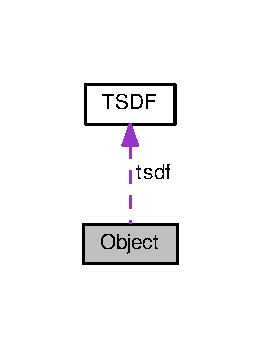
\includegraphics[width=125pt]{classObject__coll__graph}
\end{center}
\end{figure}
\subsection*{Public Member Functions}
\begin{DoxyCompactItemize}
\item 
\hyperlink{classObject_a8710a1b07956b7eadc6b05563fbb6016}{Object} (Key\+Frame $\ast$p\+KF, cv\+::\+Rect Box, cv\+::\+Mat imD, cv\+::\+Mat K, int Sensor)
\item 
\hyperlink{classObject_ae8f5483f459e46687bd01e6f9977afd3}{$\sim$\+Object} ()
\item 
\mbox{\Hypertarget{classObject_a84c579c83ad0e713014dd9b2a4bf1d81}\label{classObject_a84c579c83ad0e713014dd9b2a4bf1d81}} 
void {\bfseries Set\+Object\+Params} (float Prob\+Thd, float Min\+Object\+Points, int Height, int Width, float Min\+Depth, float Max\+Depth, float Dist, float Res)
\item 
void \hyperlink{classObject_a6661c15e096fc5ec5b6eba0eda114ac8}{Add\+Key\+Frame} (Key\+Frame $\ast$p\+KF)
\item 
void \hyperlink{classObject_a0272ba2a458346ce9e53fa0fba7799bd}{Add\+Object\+Point} (\hyperlink{classObjectPoint}{Object\+Point} $\ast$p\+MP)
\item 
vector$<$ Key\+Frame $\ast$ $>$ \hyperlink{classObject_ad2535d39e437bf0ea9ff663dbfd3b7d0}{Get\+All\+Key\+Frames} ()
\item 
vector$<$ \hyperlink{classObjectPoint}{Object\+Point} $\ast$ $>$ \hyperlink{classObject_a53b5db01428c4bcf2b54c27b0074257f}{Get\+All\+Object\+Points} ()
\item 
Key\+Frame $\ast$ \hyperlink{classObject_a3513873d737b0557c12c47c19ae2c291}{Get\+Reference\+Key\+Frame} ()
\item 
map$<$ Key\+Frame $\ast$, size\+\_\+t $>$ \hyperlink{classObject_ab17d7f60abbec82a3b45fdf322ea472e}{Get\+Observations} ()
\item 
int \hyperlink{classObject_a3b40498cabe036689eff2862e1fd8143}{Observations} ()
\item 
void \hyperlink{classObject_a1e7dbe097a891bee611dd36d64b5de64}{Add\+Observation} (Key\+Frame $\ast$p\+KF, size\+\_\+t idx)
\item 
void \hyperlink{classObject_a2f6308e77b95e3302a2f60c838839a20}{Erase\+Observation} (Key\+Frame $\ast$p\+KF)
\item 
void \hyperlink{classObject_ad585053a0c8b020a262c75fbd8c9d428}{Add\+Contour} (const Contour \&cnt)
\item 
Contour \hyperlink{classObject_a0e1e343172b51146a8e1af92ba2938d1}{Get\+Contour} (size\+\_\+t idx)
\item 
Contour \hyperlink{classObject_a8295fd33f9ebe850dbfef7b1f70f326d}{Get\+Contour} (Key\+Frame $\ast$KF)
\item 
size\+\_\+t \hyperlink{classObject_a211d9a8ea1cfbc9a3bc766b76e5d41be}{Get\+Number\+Of\+Contours} ()
\item 
void \hyperlink{classObject_a93f6229c59ae6f435b0a31ee285740ae}{Add\+Bounding\+Box} (const cv\+::\+Rect \&box)
\item 
void \hyperlink{classObject_ad680f6b7841320d67f6caf8813dc7aeb}{Set\+Label} (const std\+::string \&label)
\item 
string \hyperlink{classObject_ab60f1df2e7bd47cdfb77a529d5ad6c69}{Get\+Label} ()
\item 
void \hyperlink{classObject_a92f56ff635e752ffa2674596c8f7c1ae}{Update\+Score} (const double score)
\item 
double \hyperlink{classObject_a440178c130d1b50d232d9b96510e45a6}{Get\+Score} ()
\item 
bool \hyperlink{classObject_a38c47e88eb887dc62031e1c817e5fead}{Is\+In\+Object} (\hyperlink{classObjectPoint}{Object\+Point} $\ast$MP)
\item 
bool \hyperlink{classObject_ad4cb82b18bd457d631cb79cec0db98ac}{Has\+Enough\+Object\+Points} ()
\item 
int \hyperlink{classObject_a9fbecce492d60540c9d3fa2f81773552}{Get\+Max\+Observations} ()
\item 
cv\+::\+Point \hyperlink{classObject_a38bd011f1b615252420ae2e89d786205}{Project\+Object\+Point} (\hyperlink{classObjectPoint}{Object\+Point} $\ast$MP, Key\+Frame $\ast$KF)
\item 
void \hyperlink{classObject_a419bf8497ede00f30dd9ebacaac18987}{Add\+New\+Object\+Points} (Contour mask\+Contour, const cv\+::\+Mat \&im\+Depth, Key\+Frame $\ast$KF, float score)
\item 
\mbox{\Hypertarget{classObject_a221ae11d61c3ef7a7f80bde2f8d9290a}\label{classObject_a221ae11d61c3ef7a7f80bde2f8d9290a}} 
void {\bfseries Add\+New\+Object\+Points} (Contour mask\+Contour, const std\+::vector$<$ std\+::vector$<$ cv\+::\+Point $>$ $>$ \&clusters, const cv\+::\+Mat \&im\+Depth, Key\+Frame $\ast$KF, float score)
\item 
\mbox{\Hypertarget{classObject_a531db2d7eb149102750890f7aab97de2}\label{classObject_a531db2d7eb149102750890f7aab97de2}} 
void {\bfseries Add\+Segment} (Contour mask\+Contour, const cv\+::\+Mat \&im\+Depth, Key\+Frame $\ast$KF, float score)
\item 
\mbox{\Hypertarget{classObject_ac6b4a93f2ab97692c70c5c54ecc1628e}\label{classObject_ac6b4a93f2ab97692c70c5c54ecc1628e}} 
void {\bfseries Add\+Segment} (const std\+::vector$<$ cv\+::\+Point $>$ \&cluster, const cv\+::\+Mat \&im\+Depth, Key\+Frame $\ast$KF, float score)
\item 
void \hyperlink{classObject_a3f843dde478cc5150746d4bc3a8399f8}{Check\+Object\+Points} (Key\+Frame $\ast$K\+F2)
\item 
void \hyperlink{classObject_a438ac9db297561c832a416b304e40e87}{Integrate} (cv\+::\+Mat im\+R\+GB, cv\+::\+Mat imD, cv\+::\+Mat T)
\item 
void \hyperlink{classObject_a2994e04dbefd498087ad3f5a0ed41057}{Set\+Bad\+Flag} ()
\item 
bool \hyperlink{classObject_a3125138275bf5ab9ea78073b18a4f7c7}{is\+Bad} ()
\item 
\mbox{\Hypertarget{classObject_a8ef91a15b2f4de4f4ccaeb2020ff2ae0}\label{classObject_a8ef91a15b2f4de4f4ccaeb2020ff2ae0}} 
std\+::vector$<$ cv\+::\+Point $>$ {\bfseries Get2d\+Features} (Key\+Frame $\ast$KF, const cv\+::\+Mat \&im\+Depth)
\item 
\mbox{\Hypertarget{classObject_a0c56ad377cdad098ae40b9d6117bda7b}\label{classObject_a0c56ad377cdad098ae40b9d6117bda7b}} 
void {\bfseries Save\+To\+File} (const std\+::string \&ext)
\end{DoxyCompactItemize}
\subsection*{Static Public Member Functions}
\begin{DoxyCompactItemize}
\item 
static bool \hyperlink{classObject_aae2511e9146551564784a5841e104aac}{l\+Id} (\hyperlink{classObject}{Object} $\ast$p\+M\+O1, \hyperlink{classObject}{Object} $\ast$p\+M\+O2)
\end{DoxyCompactItemize}
\subsection*{Public Attributes}
\begin{DoxyCompactItemize}
\item 
\mbox{\Hypertarget{classObject_ab70072eb97a2eb29253c2fd3f329fd29}\label{classObject_ab70072eb97a2eb29253c2fd3f329fd29}} 
long unsigned int \hyperlink{classObject_ab70072eb97a2eb29253c2fd3f329fd29}{mn\+Id}
\begin{DoxyCompactList}\small\item\em Current \hyperlink{classObject}{Object} Id. \end{DoxyCompactList}\item 
\mbox{\Hypertarget{classObject_ab066f4ba169bd2879bcb8eddcb8b3d66}\label{classObject_ab066f4ba169bd2879bcb8eddcb8b3d66}} 
int \hyperlink{classObject_ab066f4ba169bd2879bcb8eddcb8b3d66}{n\+Obs}
\begin{DoxyCompactList}\small\item\em number of Countours in the object \end{DoxyCompactList}\item 
\mbox{\Hypertarget{classObject_aa7c1b54a6cbaa078bc42d2bfd8cd3ab4}\label{classObject_aa7c1b54a6cbaa078bc42d2bfd8cd3ab4}} 
int \hyperlink{classObject_aa7c1b54a6cbaa078bc42d2bfd8cd3ab4}{mn\+Tracks}
\begin{DoxyCompactList}\small\item\em number of Object\+Points in the object \end{DoxyCompactList}\item 
\mbox{\Hypertarget{classObject_a44e0ae2123a49d8cabbdb5899a26ab33}\label{classObject_a44e0ae2123a49d8cabbdb5899a26ab33}} 
float {\bfseries m\+Red}
\item 
\mbox{\Hypertarget{classObject_a4ebfd930ce71fb5b17fa2f2c2be8addb}\label{classObject_a4ebfd930ce71fb5b17fa2f2c2be8addb}} 
float {\bfseries m\+Green}
\item 
\mbox{\Hypertarget{classObject_a3d953a4509afe458053efc9d46cc5a9f}\label{classObject_a3d953a4509afe458053efc9d46cc5a9f}} 
float {\bfseries m\+Blue}
\end{DoxyCompactItemize}
\subsection*{Static Public Attributes}
\begin{DoxyCompactItemize}
\item 
\mbox{\Hypertarget{classObject_a3d8629d7d3aaeb68de1a5582260d7537}\label{classObject_a3d8629d7d3aaeb68de1a5582260d7537}} 
static long unsigned int \hyperlink{classObject_a3d8629d7d3aaeb68de1a5582260d7537}{n\+Next\+Id} =0
\begin{DoxyCompactList}\small\item\em Next \hyperlink{classObject}{Object} Id. \end{DoxyCompactList}\end{DoxyCompactItemize}
\subsection*{Protected Member Functions}
\begin{DoxyCompactItemize}
\item 
\mbox{\Hypertarget{classObject_a6510cecb692aac1ac052cd35c01fb033}\label{classObject_a6510cecb692aac1ac052cd35c01fb033}} 
float {\bfseries Random\+Float} ()
\end{DoxyCompactItemize}
\subsection*{Protected Attributes}
\begin{DoxyCompactItemize}
\item 
\mbox{\Hypertarget{classObject_a76ab01f0e8d22cd32a6562a00495c59b}\label{classObject_a76ab01f0e8d22cd32a6562a00495c59b}} 
std\+::set$<$ Key\+Frame $\ast$ $>$ \hyperlink{classObject_a76ab01f0e8d22cd32a6562a00495c59b}{msp\+Key\+Frames}
\begin{DoxyCompactList}\small\item\em A pointer to protected set of Key\+Frame seeing this object. \end{DoxyCompactList}\item 
\mbox{\Hypertarget{classObject_a068c5f6a016148e715eca6c4e05d42c6}\label{classObject_a068c5f6a016148e715eca6c4e05d42c6}} 
std\+::set$<$ \hyperlink{classObjectPoint}{Object\+Point} $\ast$ $>$ \hyperlink{classObject_a068c5f6a016148e715eca6c4e05d42c6}{msp\+Object\+Points}
\begin{DoxyCompactList}\small\item\em A pointer to protected set of \hyperlink{classObjectPoint}{Object\+Point} belonging to this object. \end{DoxyCompactList}\item 
\mbox{\Hypertarget{classObject_a09d584c9e2f1be37fbffd0983c048d37}\label{classObject_a09d584c9e2f1be37fbffd0983c048d37}} 
Key\+Frame $\ast$ \hyperlink{classObject_a09d584c9e2f1be37fbffd0983c048d37}{mp\+Ref\+KF}
\begin{DoxyCompactList}\small\item\em Reference Key\+Frame. \end{DoxyCompactList}\item 
\mbox{\Hypertarget{classObject_a066e5319421d737297fc3983741c689f}\label{classObject_a066e5319421d737297fc3983741c689f}} 
std\+::vector$<$ Contour $>$ \hyperlink{classObject_a066e5319421d737297fc3983741c689f}{mvp\+Contours}
\begin{DoxyCompactList}\small\item\em A vector of protected object contours. \end{DoxyCompactList}\item 
\mbox{\Hypertarget{classObject_a36f268ec71e51829dd08acde6e7870fa}\label{classObject_a36f268ec71e51829dd08acde6e7870fa}} 
std\+::vector$<$ cv\+::\+Rect $>$ \hyperlink{classObject_a36f268ec71e51829dd08acde6e7870fa}{mvp\+Bounding\+Boxes}
\begin{DoxyCompactList}\small\item\em A vector of protected object bounding boxes. \end{DoxyCompactList}\item 
\mbox{\Hypertarget{classObject_ac908f68b5c3b6dcd4b85e4c104d8da1e}\label{classObject_ac908f68b5c3b6dcd4b85e4c104d8da1e}} 
std\+::vector$<$ std\+::vector$<$ cv\+::\+Point $>$ $>$ \hyperlink{classObject_ac908f68b5c3b6dcd4b85e4c104d8da1e}{mvp\+Segments}
\begin{DoxyCompactList}\small\item\em A vector of protected object segments. \end{DoxyCompactList}\item 
\mbox{\Hypertarget{classObject_ae4d7dda62f7f9c2de88dc033237a33a9}\label{classObject_ae4d7dda62f7f9c2de88dc033237a33a9}} 
std\+::string \hyperlink{classObject_ae4d7dda62f7f9c2de88dc033237a33a9}{ms\+Label}
\begin{DoxyCompactList}\small\item\em An object label (string) \end{DoxyCompactList}\item 
\mbox{\Hypertarget{classObject_a52bd65e542dc41796db6724b4611f8dd}\label{classObject_a52bd65e542dc41796db6724b4611f8dd}} 
double \hyperlink{classObject_a52bd65e542dc41796db6724b4611f8dd}{mn\+Score}
\begin{DoxyCompactList}\small\item\em An object classification score (double) \end{DoxyCompactList}\item 
\mbox{\Hypertarget{classObject_a29e81947a25883b9e7fdb3f5c4a84076}\label{classObject_a29e81947a25883b9e7fdb3f5c4a84076}} 
std\+::map$<$ Key\+Frame $\ast$, size\+\_\+t $>$ \hyperlink{classObject_a29e81947a25883b9e7fdb3f5c4a84076}{m\+Observations}
\begin{DoxyCompactList}\small\item\em Keyframes observing the contour and associated index in keyframe-\/$>$mvp\+Contours. \end{DoxyCompactList}\item 
\mbox{\Hypertarget{classObject_a8c4672ce0a21fe301c5f11419bda84d0}\label{classObject_a8c4672ce0a21fe301c5f11419bda84d0}} 
bool \hyperlink{classObject_a8c4672ce0a21fe301c5f11419bda84d0}{mb\+Bad}
\begin{DoxyCompactList}\small\item\em Bad flag (we do not currently erase \hyperlink{classObjectPoint}{Object\+Point} from memory) \end{DoxyCompactList}\item 
\mbox{\Hypertarget{classObject_a4cc6b61d250e200e2ec5eeccc1745b79}\label{classObject_a4cc6b61d250e200e2ec5eeccc1745b79}} 
size\+\_\+t \hyperlink{classObject_a4cc6b61d250e200e2ec5eeccc1745b79}{md\+Min\+Points\+Count}
\begin{DoxyCompactList}\small\item\em Minimum number of \hyperlink{classObjectPoint}{Object\+Point} an object should allowed to have inorder to be included into the inventory. \end{DoxyCompactList}\item 
\mbox{\Hypertarget{classObject_af7eada6b6f8f5c6d7c52ba96f9c6b0d2}\label{classObject_af7eada6b6f8f5c6d7c52ba96f9c6b0d2}} 
\hyperlink{classTSDF}{T\+S\+DF} $\ast$ \hyperlink{classObject_af7eada6b6f8f5c6d7c52ba96f9c6b0d2}{tsdf}
\begin{DoxyCompactList}\small\item\em A pointer to an object \hyperlink{classTSDF}{T\+S\+DF}. \end{DoxyCompactList}\item 
\mbox{\Hypertarget{classObject_a6d8dfe87d2bbcb734681939b0c54aa86}\label{classObject_a6d8dfe87d2bbcb734681939b0c54aa86}} 
int \hyperlink{classObject_a6d8dfe87d2bbcb734681939b0c54aa86}{mn\+Height}
\begin{DoxyCompactList}\small\item\em An object depth image heights. \end{DoxyCompactList}\item 
\mbox{\Hypertarget{classObject_a32d2930a06f611ed2a7cbff167736eeb}\label{classObject_a32d2930a06f611ed2a7cbff167736eeb}} 
int \hyperlink{classObject_a32d2930a06f611ed2a7cbff167736eeb}{mn\+Width}
\begin{DoxyCompactList}\small\item\em An object depth image width. \end{DoxyCompactList}\item 
\mbox{\Hypertarget{classObject_a98a79df663772f156d9dcb10f5de3dfe}\label{classObject_a98a79df663772f156d9dcb10f5de3dfe}} 
float \hyperlink{classObject_a98a79df663772f156d9dcb10f5de3dfe}{mn\+Min\+Depth}
\begin{DoxyCompactList}\small\item\em Minimum perceived depth. \end{DoxyCompactList}\item 
\mbox{\Hypertarget{classObject_ad8d8002cdaacd83e40034ab1b5f7d911}\label{classObject_ad8d8002cdaacd83e40034ab1b5f7d911}} 
float \hyperlink{classObject_ad8d8002cdaacd83e40034ab1b5f7d911}{mn\+Max\+Depth}
\begin{DoxyCompactList}\small\item\em Maximum perceived depth. \end{DoxyCompactList}\item 
\mbox{\Hypertarget{classObject_ae5eea391874be8f3eb266d81e17f2226}\label{classObject_ae5eea391874be8f3eb266d81e17f2226}} 
float \hyperlink{classObject_ae5eea391874be8f3eb266d81e17f2226}{mn\+Res}
\begin{DoxyCompactList}\small\item\em \hyperlink{classObject}{Object} resolution. \end{DoxyCompactList}\item 
\mbox{\Hypertarget{classObject_a0ec14c1b27b32ab767db6260afeea589}\label{classObject_a0ec14c1b27b32ab767db6260afeea589}} 
float \hyperlink{classObject_a0ec14c1b27b32ab767db6260afeea589}{mn\+Dist}
\begin{DoxyCompactList}\small\item\em Point-\/to-\/polygon test. \end{DoxyCompactList}\item 
\mbox{\Hypertarget{classObject_a378aecb006051eee845c107994cfadd8}\label{classObject_a378aecb006051eee845c107994cfadd8}} 
float {\bfseries m\+Prob\+Thd}
\item 
\mbox{\Hypertarget{classObject_ab648d7302834a422496368e5d7532ddb}\label{classObject_ab648d7302834a422496368e5d7532ddb}} 
int {\bfseries m\+Sensor}
\item 
cv\+::\+Mat \hyperlink{classObject_a9cd6392d2ccce339a115090f02275e12}{mK}
\begin{DoxyCompactList}\small\item\em Camera intrinsic parameters (T\+UM) \end{DoxyCompactList}\item 
\mbox{\Hypertarget{classObject_a3ae09a637a49579e135cd031307d6f9c}\label{classObject_a3ae09a637a49579e135cd031307d6f9c}} 
cv\+::\+Mat \hyperlink{classObject_a3ae09a637a49579e135cd031307d6f9c}{m\+Dist\+Coef} = (cv\+::\+Mat\+\_\+$<$float$>$(4,1) $<$$<$ 0, 0, 0, 0)
\begin{DoxyCompactList}\small\item\em Camera lense distortion parameters. \end{DoxyCompactList}\item 
\mbox{\Hypertarget{classObject_af22d050229447532f43c27561a2e6a2c}\label{classObject_af22d050229447532f43c27561a2e6a2c}} 
std\+::mutex {\bfseries m\+Mutex\+Object}
\end{DoxyCompactItemize}


\subsection{Detailed Description}
A definition of an object in the inventory. 

\begin{DoxyAuthor}{Author}
Tariq Abuhashim 
\end{DoxyAuthor}
\begin{DoxyDate}{Date}
August 2019 
\end{DoxyDate}


\subsection{Constructor \& Destructor Documentation}
\mbox{\Hypertarget{classObject_a8710a1b07956b7eadc6b05563fbb6016}\label{classObject_a8710a1b07956b7eadc6b05563fbb6016}} 
\index{Object@{Object}!Object@{Object}}
\index{Object@{Object}!Object@{Object}}
\subsubsection{\texorpdfstring{Object()}{Object()}}
{\footnotesize\ttfamily Object\+::\+Object (\begin{DoxyParamCaption}\item[{Key\+Frame $\ast$}]{p\+KF,  }\item[{cv\+::\+Rect}]{Box,  }\item[{cv\+::\+Mat}]{imD,  }\item[{cv\+::\+Mat}]{K,  }\item[{int}]{Sensor }\end{DoxyParamCaption})}

\hyperlink{classObject}{Object} constructor 
\begin{DoxyParams}{Parameters}
{\em h} & height of the object depth image (called to initialise an object and its \hyperlink{classTSDF}{T\+S\+DF}) \\
\hline
{\em w} & width of the object depth image (called to initialise an object and its \hyperlink{classTSDF}{T\+S\+DF}) \\
\hline
\end{DoxyParams}
\mbox{\Hypertarget{classObject_ae8f5483f459e46687bd01e6f9977afd3}\label{classObject_ae8f5483f459e46687bd01e6f9977afd3}} 
\index{Object@{Object}!````~Object@{$\sim$\+Object}}
\index{````~Object@{$\sim$\+Object}!Object@{Object}}
\subsubsection{\texorpdfstring{$\sim$\+Object()}{~Object()}}
{\footnotesize\ttfamily Object\+::$\sim$\+Object (\begin{DoxyParamCaption}{ }\end{DoxyParamCaption})}

\hyperlink{classObject}{Object} destructor (called to delete an object \hyperlink{classTSDF}{T\+S\+DF} from memory) 

\subsection{Member Function Documentation}
\mbox{\Hypertarget{classObject_a93f6229c59ae6f435b0a31ee285740ae}\label{classObject_a93f6229c59ae6f435b0a31ee285740ae}} 
\index{Object@{Object}!Add\+Bounding\+Box@{Add\+Bounding\+Box}}
\index{Add\+Bounding\+Box@{Add\+Bounding\+Box}!Object@{Object}}
\subsubsection{\texorpdfstring{Add\+Bounding\+Box()}{AddBoundingBox()}}
{\footnotesize\ttfamily void Object\+::\+Add\+Bounding\+Box (\begin{DoxyParamCaption}\item[{const cv\+::\+Rect \&}]{box }\end{DoxyParamCaption})}

Adds an object bounding box. 
\begin{DoxyParams}{Parameters}
{\em box} & the current bounding box to be added. \\
\hline
\end{DoxyParams}
\mbox{\Hypertarget{classObject_ad585053a0c8b020a262c75fbd8c9d428}\label{classObject_ad585053a0c8b020a262c75fbd8c9d428}} 
\index{Object@{Object}!Add\+Contour@{Add\+Contour}}
\index{Add\+Contour@{Add\+Contour}!Object@{Object}}
\subsubsection{\texorpdfstring{Add\+Contour()}{AddContour()}}
{\footnotesize\ttfamily void Object\+::\+Add\+Contour (\begin{DoxyParamCaption}\item[{const Contour \&}]{cnt }\end{DoxyParamCaption})}

Adds a contour obsevation into the object vector of contours (mvp\+Contours) 
\begin{DoxyParams}{Parameters}
{\em cnt} & the current contour \\
\hline
\end{DoxyParams}
\mbox{\Hypertarget{classObject_a6661c15e096fc5ec5b6eba0eda114ac8}\label{classObject_a6661c15e096fc5ec5b6eba0eda114ac8}} 
\index{Object@{Object}!Add\+Key\+Frame@{Add\+Key\+Frame}}
\index{Add\+Key\+Frame@{Add\+Key\+Frame}!Object@{Object}}
\subsubsection{\texorpdfstring{Add\+Key\+Frame()}{AddKeyFrame()}}
{\footnotesize\ttfamily void Object\+::\+Add\+Key\+Frame (\begin{DoxyParamCaption}\item[{Key\+Frame $\ast$}]{p\+KF }\end{DoxyParamCaption})}

A function that includes a Key\+Frame into the set of Key\+Frames where the object is visible. 
\begin{DoxyParams}{Parameters}
{\em p\+KF} & the current Key\+Frame to add \\
\hline
\end{DoxyParams}
\mbox{\Hypertarget{classObject_a419bf8497ede00f30dd9ebacaac18987}\label{classObject_a419bf8497ede00f30dd9ebacaac18987}} 
\index{Object@{Object}!Add\+New\+Object\+Points@{Add\+New\+Object\+Points}}
\index{Add\+New\+Object\+Points@{Add\+New\+Object\+Points}!Object@{Object}}
\subsubsection{\texorpdfstring{Add\+New\+Object\+Points()}{AddNewObjectPoints()}}
{\footnotesize\ttfamily void Object\+::\+Add\+New\+Object\+Points (\begin{DoxyParamCaption}\item[{Contour}]{mask\+Contour,  }\item[{const cv\+::\+Mat \&}]{im\+Depth,  }\item[{Key\+Frame $\ast$}]{KF,  }\item[{float}]{score }\end{DoxyParamCaption})}

Iterates through all map points and add points the agrees with the current contour into the object 
\begin{DoxyParams}{Parameters}
{\em mask\+Contour} & \hyperlink{classObject}{Object} contours \\
\hline
{\em im\+Depth} & the current Key\+Frame depth image \\
\hline
{\em KF} & pointer to the current O\+R\+B\+S\+L\+A\+M2\+::\+Key\+Frame \\
\hline
\end{DoxyParams}
\mbox{\Hypertarget{classObject_a0272ba2a458346ce9e53fa0fba7799bd}\label{classObject_a0272ba2a458346ce9e53fa0fba7799bd}} 
\index{Object@{Object}!Add\+Object\+Point@{Add\+Object\+Point}}
\index{Add\+Object\+Point@{Add\+Object\+Point}!Object@{Object}}
\subsubsection{\texorpdfstring{Add\+Object\+Point()}{AddObjectPoint()}}
{\footnotesize\ttfamily void Object\+::\+Add\+Object\+Point (\begin{DoxyParamCaption}\item[{\hyperlink{classObjectPoint}{Object\+Point} $\ast$}]{p\+MP }\end{DoxyParamCaption})}

A function that includes a \hyperlink{classObjectPoint}{Object\+Point} into the set of Object\+Points that belongs to an object is the map. Hence, this pointer also links the object to 
\begin{DoxyParams}{Parameters}
{\em p\+MP} & the current \hyperlink{classObjectPoint}{Object\+Point} to add (mv\+Keys) in its (KF) -\/ Refer to O\+R\+B\+S\+L\+A\+M2\+::\+Key\+Frame for details \\
\hline
\end{DoxyParams}
\mbox{\Hypertarget{classObject_a1e7dbe097a891bee611dd36d64b5de64}\label{classObject_a1e7dbe097a891bee611dd36d64b5de64}} 
\index{Object@{Object}!Add\+Observation@{Add\+Observation}}
\index{Add\+Observation@{Add\+Observation}!Object@{Object}}
\subsubsection{\texorpdfstring{Add\+Observation()}{AddObservation()}}
{\footnotesize\ttfamily void Object\+::\+Add\+Observation (\begin{DoxyParamCaption}\item[{Key\+Frame $\ast$}]{p\+KF,  }\item[{size\+\_\+t}]{idx }\end{DoxyParamCaption})}

Adds details of a contour obsevation into the object. This function is used to know which contour in mvp\+Contours is in KF. The implementation allows a contour to be called by either its Key\+Frame or index. 
\begin{DoxyParams}{Parameters}
{\em p\+KF} & the current Key\+Frame where the contour is \\
\hline
{\em idx} & the index of the countour in the object. \\
\hline
\end{DoxyParams}
\mbox{\Hypertarget{classObject_a3f843dde478cc5150746d4bc3a8399f8}\label{classObject_a3f843dde478cc5150746d4bc3a8399f8}} 
\index{Object@{Object}!Check\+Object\+Points@{Check\+Object\+Points}}
\index{Check\+Object\+Points@{Check\+Object\+Points}!Object@{Object}}
\subsubsection{\texorpdfstring{Check\+Object\+Points()}{CheckObjectPoints()}}
{\footnotesize\ttfamily void Object\+::\+Check\+Object\+Points (\begin{DoxyParamCaption}\item[{Key\+Frame $\ast$}]{K\+F2 }\end{DoxyParamCaption})}

Iterates through all object points and verifies the good and bad ones, then deletes/flags the bad ones. 
\begin{DoxyParams}{Parameters}
{\em K\+F2} & pointer to the current O\+R\+B\+S\+L\+A\+M2\+::\+Key\+Frame \\
\hline
\end{DoxyParams}
\mbox{\Hypertarget{classObject_a2f6308e77b95e3302a2f60c838839a20}\label{classObject_a2f6308e77b95e3302a2f60c838839a20}} 
\index{Object@{Object}!Erase\+Observation@{Erase\+Observation}}
\index{Erase\+Observation@{Erase\+Observation}!Object@{Object}}
\subsubsection{\texorpdfstring{Erase\+Observation()}{EraseObservation()}}
{\footnotesize\ttfamily void Object\+::\+Erase\+Observation (\begin{DoxyParamCaption}\item[{Key\+Frame $\ast$}]{p\+KF }\end{DoxyParamCaption})}

Removes a contour obsevation into the object. This function is used to delete the contour with index (idx) which is visible in Key\+Frame (KF). The contour is deleted from mvp\+Contours. 
\begin{DoxyParams}{Parameters}
{\em p\+KF} & the current Key\+Frame where the contour is \\
\hline
\end{DoxyParams}
\mbox{\Hypertarget{classObject_ad2535d39e437bf0ea9ff663dbfd3b7d0}\label{classObject_ad2535d39e437bf0ea9ff663dbfd3b7d0}} 
\index{Object@{Object}!Get\+All\+Key\+Frames@{Get\+All\+Key\+Frames}}
\index{Get\+All\+Key\+Frames@{Get\+All\+Key\+Frames}!Object@{Object}}
\subsubsection{\texorpdfstring{Get\+All\+Key\+Frames()}{GetAllKeyFrames()}}
{\footnotesize\ttfamily vector$<$ Key\+Frame $\ast$ $>$ Object\+::\+Get\+All\+Key\+Frames (\begin{DoxyParamCaption}{ }\end{DoxyParamCaption})}

Returns a vector of all Key\+Frame pointers with an the object contour observations \mbox{\Hypertarget{classObject_a53b5db01428c4bcf2b54c27b0074257f}\label{classObject_a53b5db01428c4bcf2b54c27b0074257f}} 
\index{Object@{Object}!Get\+All\+Object\+Points@{Get\+All\+Object\+Points}}
\index{Get\+All\+Object\+Points@{Get\+All\+Object\+Points}!Object@{Object}}
\subsubsection{\texorpdfstring{Get\+All\+Object\+Points()}{GetAllObjectPoints()}}
{\footnotesize\ttfamily vector$<$ \hyperlink{classObjectPoint}{Object\+Point} $\ast$ $>$ Object\+::\+Get\+All\+Object\+Points (\begin{DoxyParamCaption}{ }\end{DoxyParamCaption})}

Returns a vector of all \hyperlink{classObjectPoint}{Object\+Point} pointers of the object in the map \mbox{\Hypertarget{classObject_a0e1e343172b51146a8e1af92ba2938d1}\label{classObject_a0e1e343172b51146a8e1af92ba2938d1}} 
\index{Object@{Object}!Get\+Contour@{Get\+Contour}}
\index{Get\+Contour@{Get\+Contour}!Object@{Object}}
\subsubsection{\texorpdfstring{Get\+Contour()}{GetContour()}\hspace{0.1cm}{\footnotesize\ttfamily [1/2]}}
{\footnotesize\ttfamily Contour Object\+::\+Get\+Contour (\begin{DoxyParamCaption}\item[{size\+\_\+t}]{idx }\end{DoxyParamCaption})}

Returns a contour observation by index (idx). 
\begin{DoxyParams}{Parameters}
{\em idx} & is the called contour index \\
\hline
\end{DoxyParams}
\mbox{\Hypertarget{classObject_a8295fd33f9ebe850dbfef7b1f70f326d}\label{classObject_a8295fd33f9ebe850dbfef7b1f70f326d}} 
\index{Object@{Object}!Get\+Contour@{Get\+Contour}}
\index{Get\+Contour@{Get\+Contour}!Object@{Object}}
\subsubsection{\texorpdfstring{Get\+Contour()}{GetContour()}\hspace{0.1cm}{\footnotesize\ttfamily [2/2]}}
{\footnotesize\ttfamily Contour Object\+::\+Get\+Contour (\begin{DoxyParamCaption}\item[{Key\+Frame $\ast$}]{KF }\end{DoxyParamCaption})}

Returns a contour observation by Key\+Frame (KF). This method is more reliable at linking contours to Key\+Frames than using indexing. 
\begin{DoxyParams}{Parameters}
{\em KF} & is a pointer to Key\+Frame viewing the object. \\
\hline
\end{DoxyParams}
\mbox{\Hypertarget{classObject_ab60f1df2e7bd47cdfb77a529d5ad6c69}\label{classObject_ab60f1df2e7bd47cdfb77a529d5ad6c69}} 
\index{Object@{Object}!Get\+Label@{Get\+Label}}
\index{Get\+Label@{Get\+Label}!Object@{Object}}
\subsubsection{\texorpdfstring{Get\+Label()}{GetLabel()}}
{\footnotesize\ttfamily std\+::string Object\+::\+Get\+Label (\begin{DoxyParamCaption}{ }\end{DoxyParamCaption})}

Returns the current classification label of the object. \mbox{\Hypertarget{classObject_a9fbecce492d60540c9d3fa2f81773552}\label{classObject_a9fbecce492d60540c9d3fa2f81773552}} 
\index{Object@{Object}!Get\+Max\+Observations@{Get\+Max\+Observations}}
\index{Get\+Max\+Observations@{Get\+Max\+Observations}!Object@{Object}}
\subsubsection{\texorpdfstring{Get\+Max\+Observations()}{GetMaxObservations()}}
{\footnotesize\ttfamily int Object\+::\+Get\+Max\+Observations (\begin{DoxyParamCaption}{ }\end{DoxyParamCaption})}

Returns the maximum (or total) number of 2D point observations that matches the object contours This reflects how many times a \hyperlink{classObjectPoint}{Object\+Point} has agreed with this object contours. \mbox{\Hypertarget{classObject_a211d9a8ea1cfbc9a3bc766b76e5d41be}\label{classObject_a211d9a8ea1cfbc9a3bc766b76e5d41be}} 
\index{Object@{Object}!Get\+Number\+Of\+Contours@{Get\+Number\+Of\+Contours}}
\index{Get\+Number\+Of\+Contours@{Get\+Number\+Of\+Contours}!Object@{Object}}
\subsubsection{\texorpdfstring{Get\+Number\+Of\+Contours()}{GetNumberOfContours()}}
{\footnotesize\ttfamily size\+\_\+t Object\+::\+Get\+Number\+Of\+Contours (\begin{DoxyParamCaption}{ }\end{DoxyParamCaption})}

Returns the total number of object contours in the dataset \mbox{\Hypertarget{classObject_ab17d7f60abbec82a3b45fdf322ea472e}\label{classObject_ab17d7f60abbec82a3b45fdf322ea472e}} 
\index{Object@{Object}!Get\+Observations@{Get\+Observations}}
\index{Get\+Observations@{Get\+Observations}!Object@{Object}}
\subsubsection{\texorpdfstring{Get\+Observations()}{GetObservations()}}
{\footnotesize\ttfamily std\+::map$<$ Key\+Frame $\ast$, size\+\_\+t $>$ Object\+::\+Get\+Observations (\begin{DoxyParamCaption}{ }\end{DoxyParamCaption})}

Returns a map of Keyframes observing the contour and associated index in keyframe \mbox{\Hypertarget{classObject_a3513873d737b0557c12c47c19ae2c291}\label{classObject_a3513873d737b0557c12c47c19ae2c291}} 
\index{Object@{Object}!Get\+Reference\+Key\+Frame@{Get\+Reference\+Key\+Frame}}
\index{Get\+Reference\+Key\+Frame@{Get\+Reference\+Key\+Frame}!Object@{Object}}
\subsubsection{\texorpdfstring{Get\+Reference\+Key\+Frame()}{GetReferenceKeyFrame()}}
{\footnotesize\ttfamily Key\+Frame $\ast$ Object\+::\+Get\+Reference\+Key\+Frame (\begin{DoxyParamCaption}{ }\end{DoxyParamCaption})}

returns a pointer to the map object reference Key\+Frame (usually the first Key\+Frame seeing object) \mbox{\Hypertarget{classObject_a440178c130d1b50d232d9b96510e45a6}\label{classObject_a440178c130d1b50d232d9b96510e45a6}} 
\index{Object@{Object}!Get\+Score@{Get\+Score}}
\index{Get\+Score@{Get\+Score}!Object@{Object}}
\subsubsection{\texorpdfstring{Get\+Score()}{GetScore()}}
{\footnotesize\ttfamily double Object\+::\+Get\+Score (\begin{DoxyParamCaption}{ }\end{DoxyParamCaption})}

Returns the current classification score of the object. \mbox{\Hypertarget{classObject_ad4cb82b18bd457d631cb79cec0db98ac}\label{classObject_ad4cb82b18bd457d631cb79cec0db98ac}} 
\index{Object@{Object}!Has\+Enough\+Object\+Points@{Has\+Enough\+Object\+Points}}
\index{Has\+Enough\+Object\+Points@{Has\+Enough\+Object\+Points}!Object@{Object}}
\subsubsection{\texorpdfstring{Has\+Enough\+Object\+Points()}{HasEnoughObjectPoints()}}
{\footnotesize\ttfamily bool Object\+::\+Has\+Enough\+Object\+Points (\begin{DoxyParamCaption}{ }\end{DoxyParamCaption})}

Verifies if an object contour contains enough 2D map points to be considered a valid object measurement. \mbox{\Hypertarget{classObject_a438ac9db297561c832a416b304e40e87}\label{classObject_a438ac9db297561c832a416b304e40e87}} 
\index{Object@{Object}!Integrate@{Integrate}}
\index{Integrate@{Integrate}!Object@{Object}}
\subsubsection{\texorpdfstring{Integrate()}{Integrate()}}
{\footnotesize\ttfamily void Object\+::\+Integrate (\begin{DoxyParamCaption}\item[{cv\+::\+Mat}]{im\+R\+GB,  }\item[{cv\+::\+Mat}]{imD,  }\item[{cv\+::\+Mat}]{T }\end{DoxyParamCaption})}

Integrates the current depth image into the object \hyperlink{classTSDF}{T\+S\+DF} \mbox{\Hypertarget{classObject_a3125138275bf5ab9ea78073b18a4f7c7}\label{classObject_a3125138275bf5ab9ea78073b18a4f7c7}} 
\index{Object@{Object}!is\+Bad@{is\+Bad}}
\index{is\+Bad@{is\+Bad}!Object@{Object}}
\subsubsection{\texorpdfstring{is\+Bad()}{isBad()}}
{\footnotesize\ttfamily bool Object\+::is\+Bad (\begin{DoxyParamCaption}{ }\end{DoxyParamCaption})}

Returns true if the object is bad (F\+I\+X\+ME\+: not implemented yet) \mbox{\Hypertarget{classObject_a38c47e88eb887dc62031e1c817e5fead}\label{classObject_a38c47e88eb887dc62031e1c817e5fead}} 
\index{Object@{Object}!Is\+In\+Object@{Is\+In\+Object}}
\index{Is\+In\+Object@{Is\+In\+Object}!Object@{Object}}
\subsubsection{\texorpdfstring{Is\+In\+Object()}{IsInObject()}}
{\footnotesize\ttfamily bool Object\+::\+Is\+In\+Object (\begin{DoxyParamCaption}\item[{\hyperlink{classObjectPoint}{Object\+Point} $\ast$}]{MP }\end{DoxyParamCaption})}

Verifies if a \hyperlink{classObjectPoint}{Object\+Point} lays inside an object contours. 
\begin{DoxyParams}{Parameters}
{\em MP} & a pointer to the current \hyperlink{classObjectPoint}{Object\+Point} to test. \\
\hline
\end{DoxyParams}
\mbox{\Hypertarget{classObject_aae2511e9146551564784a5841e104aac}\label{classObject_aae2511e9146551564784a5841e104aac}} 
\index{Object@{Object}!l\+Id@{l\+Id}}
\index{l\+Id@{l\+Id}!Object@{Object}}
\subsubsection{\texorpdfstring{l\+Id()}{lId()}}
{\footnotesize\ttfamily static bool Object\+::l\+Id (\begin{DoxyParamCaption}\item[{\hyperlink{classObject}{Object} $\ast$}]{p\+M\+O1,  }\item[{\hyperlink{classObject}{Object} $\ast$}]{p\+M\+O2 }\end{DoxyParamCaption})\hspace{0.3cm}{\ttfamily [inline]}, {\ttfamily [static]}}

Custom compare function to sort map objects using their index (mn\+Id) \mbox{\Hypertarget{classObject_a3b40498cabe036689eff2862e1fd8143}\label{classObject_a3b40498cabe036689eff2862e1fd8143}} 
\index{Object@{Object}!Observations@{Observations}}
\index{Observations@{Observations}!Object@{Object}}
\subsubsection{\texorpdfstring{Observations()}{Observations()}}
{\footnotesize\ttfamily int Object\+::\+Observations (\begin{DoxyParamCaption}{ }\end{DoxyParamCaption})}

Returns the number of contours of the objects in the dataset \mbox{\Hypertarget{classObject_a38bd011f1b615252420ae2e89d786205}\label{classObject_a38bd011f1b615252420ae2e89d786205}} 
\index{Object@{Object}!Project\+Object\+Point@{Project\+Object\+Point}}
\index{Project\+Object\+Point@{Project\+Object\+Point}!Object@{Object}}
\subsubsection{\texorpdfstring{Project\+Object\+Point()}{ProjectObjectPoint()}}
{\footnotesize\ttfamily cv\+::\+Point Object\+::\+Project\+Object\+Point (\begin{DoxyParamCaption}\item[{\hyperlink{classObjectPoint}{Object\+Point} $\ast$}]{MP,  }\item[{Key\+Frame $\ast$}]{KF }\end{DoxyParamCaption})}

Projects a 3D \hyperlink{classObjectPoint}{Object\+Point} into a 2D Key\+Frame image 
\begin{DoxyParams}{Parameters}
{\em MP} & a pointer to the current \hyperlink{classObjectPoint}{Object\+Point} \\
\hline
{\em KF} & a pointer to the current Key\+Frame \\
\hline
{\em K} & intrinsic calibration parameters \\
\hline
\end{DoxyParams}
\mbox{\Hypertarget{classObject_a2994e04dbefd498087ad3f5a0ed41057}\label{classObject_a2994e04dbefd498087ad3f5a0ed41057}} 
\index{Object@{Object}!Set\+Bad\+Flag@{Set\+Bad\+Flag}}
\index{Set\+Bad\+Flag@{Set\+Bad\+Flag}!Object@{Object}}
\subsubsection{\texorpdfstring{Set\+Bad\+Flag()}{SetBadFlag()}}
{\footnotesize\ttfamily void Object\+::\+Set\+Bad\+Flag (\begin{DoxyParamCaption}{ }\end{DoxyParamCaption})}

Sets the object bad (F\+I\+X\+ME\+: not implemented yet) \mbox{\Hypertarget{classObject_ad680f6b7841320d67f6caf8813dc7aeb}\label{classObject_ad680f6b7841320d67f6caf8813dc7aeb}} 
\index{Object@{Object}!Set\+Label@{Set\+Label}}
\index{Set\+Label@{Set\+Label}!Object@{Object}}
\subsubsection{\texorpdfstring{Set\+Label()}{SetLabel()}}
{\footnotesize\ttfamily void Object\+::\+Set\+Label (\begin{DoxyParamCaption}\item[{const std\+::string \&}]{label }\end{DoxyParamCaption})}

Sets the classification label of the object. 
\begin{DoxyParams}{Parameters}
{\em label} & the current label from \hyperlink{classMaskRCNN}{Mask\+R\+C\+NN} or label-\/fusion rule ? \\
\hline
\end{DoxyParams}
\mbox{\Hypertarget{classObject_a92f56ff635e752ffa2674596c8f7c1ae}\label{classObject_a92f56ff635e752ffa2674596c8f7c1ae}} 
\index{Object@{Object}!Update\+Score@{Update\+Score}}
\index{Update\+Score@{Update\+Score}!Object@{Object}}
\subsubsection{\texorpdfstring{Update\+Score()}{UpdateScore()}}
{\footnotesize\ttfamily void Object\+::\+Update\+Score (\begin{DoxyParamCaption}\item[{const double}]{score }\end{DoxyParamCaption})}

Updates the score of the object given most recent contour/\+Mask\+R\+C\+NN obsevations. 
\begin{DoxyParams}{Parameters}
{\em score} & the current score from \hyperlink{classMaskRCNN}{Mask\+R\+C\+NN} or score-\/fusion rule ? \\
\hline
\end{DoxyParams}


\subsection{Member Data Documentation}
\mbox{\Hypertarget{classObject_a9cd6392d2ccce339a115090f02275e12}\label{classObject_a9cd6392d2ccce339a115090f02275e12}} 
\index{Object@{Object}!mK@{mK}}
\index{mK@{mK}!Object@{Object}}
\subsubsection{\texorpdfstring{mK}{mK}}
{\footnotesize\ttfamily cv\+::\+Mat Object\+::mK\hspace{0.3cm}{\ttfamily [protected]}}



Camera intrinsic parameters (T\+UM) 

Camera intrinsic parameters (Kitti) 

The documentation for this class was generated from the following files\+:\begin{DoxyCompactItemize}
\item 
/home/mrt/\+Dev/maskrcnn\+\_\+slam\+\_\+b/include/Object.\+hpp\item 
/home/mrt/\+Dev/maskrcnn\+\_\+slam\+\_\+b/src/Object.\+cpp\end{DoxyCompactItemize}

\hypertarget{classObjectDrawer}{}\section{Object\+Drawer Class Reference}
\label{classObjectDrawer}\index{Object\+Drawer@{Object\+Drawer}}


Collaboration diagram for Object\+Drawer\+:\nopagebreak
\begin{figure}[H]
\begin{center}
\leavevmode
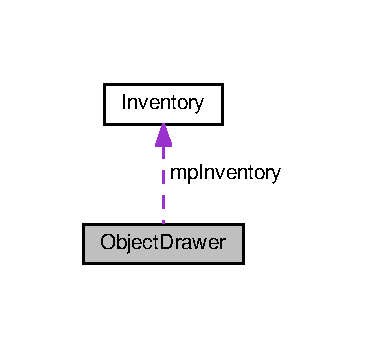
\includegraphics[width=177pt]{classObjectDrawer__coll__graph}
\end{center}
\end{figure}
\subsection*{Public Member Functions}
\begin{DoxyCompactItemize}
\item 
\mbox{\Hypertarget{classObjectDrawer_ae670d3818a6a95402aba4ccdc90b8fc0}\label{classObjectDrawer_ae670d3818a6a95402aba4ccdc90b8fc0}} 
{\bfseries Object\+Drawer} (\hyperlink{classInventory}{Inventory} $\ast$p\+Inventory, const string \&str\+Setting\+Path)
\item 
\mbox{\Hypertarget{classObjectDrawer_a4e673493a9b2545b199c61b7a5239891}\label{classObjectDrawer_a4e673493a9b2545b199c61b7a5239891}} 
void {\bfseries Draw\+Map\+Points} ()
\item 
\mbox{\Hypertarget{classObjectDrawer_a02381ea8fad3c699a213dcde13161827}\label{classObjectDrawer_a02381ea8fad3c699a213dcde13161827}} 
void {\bfseries Draw\+Key\+Frames} (const bool b\+Draw\+KF, const bool b\+Draw\+Graph)
\item 
\mbox{\Hypertarget{classObjectDrawer_ab86f02d748af2b18d68315cdfeebe13b}\label{classObjectDrawer_ab86f02d748af2b18d68315cdfeebe13b}} 
void {\bfseries Draw\+Current\+Camera} (pangolin\+::\+Open\+Gl\+Matrix \&Twc)
\item 
\mbox{\Hypertarget{classObjectDrawer_a64cdd1b62c008509af2151d2d5589c27}\label{classObjectDrawer_a64cdd1b62c008509af2151d2d5589c27}} 
void {\bfseries Set\+Current\+Camera\+Pose} (const cv\+::\+Mat \&Tcw)
\item 
\mbox{\Hypertarget{classObjectDrawer_a9e2c0acae16f47058e82a0c78a5ebe20}\label{classObjectDrawer_a9e2c0acae16f47058e82a0c78a5ebe20}} 
void {\bfseries Set\+Reference\+Key\+Frame} (Key\+Frame $\ast$p\+KF)
\item 
\mbox{\Hypertarget{classObjectDrawer_abf864858f14bd575386e18362b7b8433}\label{classObjectDrawer_abf864858f14bd575386e18362b7b8433}} 
void {\bfseries Get\+Current\+Open\+G\+L\+Camera\+Matrix} (pangolin\+::\+Open\+Gl\+Matrix \&M)
\end{DoxyCompactItemize}
\subsection*{Public Attributes}
\begin{DoxyCompactItemize}
\item 
\mbox{\Hypertarget{classObjectDrawer_a8bddfa20eefe1f70cf7fc5a0b62d7aaa}\label{classObjectDrawer_a8bddfa20eefe1f70cf7fc5a0b62d7aaa}} 
\hyperlink{classInventory}{Inventory} $\ast$ {\bfseries mp\+Inventory}
\end{DoxyCompactItemize}


The documentation for this class was generated from the following files\+:\begin{DoxyCompactItemize}
\item 
/home/mrt/\+Dev/maskrcnn\+\_\+slam\+\_\+b/include/Object\+Drawer.\+hpp\item 
/home/mrt/\+Dev/maskrcnn\+\_\+slam\+\_\+b/src/Object\+Drawer.\+cpp\end{DoxyCompactItemize}

\hypertarget{classObjectPoint}{}\section{Object\+Point Class Reference}
\label{classObjectPoint}\index{Object\+Point@{Object\+Point}}


Collaboration diagram for Object\+Point\+:\nopagebreak
\begin{figure}[H]
\begin{center}
\leavevmode
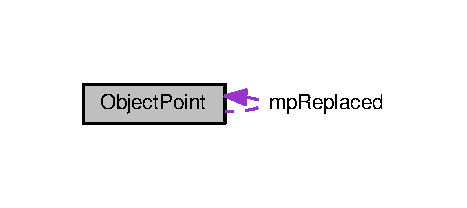
\includegraphics[width=224pt]{classObjectPoint__coll__graph}
\end{center}
\end{figure}
\subsection*{Public Member Functions}
\begin{DoxyCompactItemize}
\item 
\mbox{\Hypertarget{classObjectPoint_abe20569ffec71bce3c7798dd20098eff}\label{classObjectPoint_abe20569ffec71bce3c7798dd20098eff}} 
{\bfseries Object\+Point} (const cv\+::\+Mat \&Pos, Key\+Frame $\ast$p\+Ref\+KF)
\item 
\mbox{\Hypertarget{classObjectPoint_a9202ad0239743be43bbae9af182fed56}\label{classObjectPoint_a9202ad0239743be43bbae9af182fed56}} 
void {\bfseries Set\+World\+Pos} (const cv\+::\+Mat \&Pos)
\item 
\mbox{\Hypertarget{classObjectPoint_ae872c8a2e3ca4b541252e13555f625fb}\label{classObjectPoint_ae872c8a2e3ca4b541252e13555f625fb}} 
cv\+::\+Mat {\bfseries Get\+World\+Pos} ()
\item 
\mbox{\Hypertarget{classObjectPoint_ad543762a92802bf9fb601d208e4c007c}\label{classObjectPoint_ad543762a92802bf9fb601d208e4c007c}} 
cv\+::\+Mat {\bfseries Get\+Normal} ()
\item 
\mbox{\Hypertarget{classObjectPoint_ac205d86215aa26315881f4db4ef695b5}\label{classObjectPoint_ac205d86215aa26315881f4db4ef695b5}} 
Key\+Frame $\ast$ {\bfseries Get\+Reference\+Key\+Frame} ()
\item 
\mbox{\Hypertarget{classObjectPoint_a38d19937c25237ba87eb32e8fd2d935b}\label{classObjectPoint_a38d19937c25237ba87eb32e8fd2d935b}} 
std\+::map$<$ Key\+Frame $\ast$, size\+\_\+t $>$ {\bfseries Get\+Observations} ()
\item 
\mbox{\Hypertarget{classObjectPoint_ae7d2d3ae8c19070f2bcf41f5507ca194}\label{classObjectPoint_ae7d2d3ae8c19070f2bcf41f5507ca194}} 
int {\bfseries Observations} ()
\item 
\mbox{\Hypertarget{classObjectPoint_ade4a1f546a7dc3d0a17fd7f73b5252e5}\label{classObjectPoint_ade4a1f546a7dc3d0a17fd7f73b5252e5}} 
void {\bfseries Add\+Observation} (Key\+Frame $\ast$p\+KF, size\+\_\+t idx)
\item 
\mbox{\Hypertarget{classObjectPoint_a59da3ff3ffccde349304b779f3457254}\label{classObjectPoint_a59da3ff3ffccde349304b779f3457254}} 
void {\bfseries Erase\+Observation} (Key\+Frame $\ast$p\+KF)
\item 
\mbox{\Hypertarget{classObjectPoint_a6952d1e522571ebc982708b931006ac1}\label{classObjectPoint_a6952d1e522571ebc982708b931006ac1}} 
int {\bfseries Get\+Index\+In\+Key\+Frame} (Key\+Frame $\ast$p\+KF)
\item 
\mbox{\Hypertarget{classObjectPoint_a2f2689ae271ff5507808625c575da632}\label{classObjectPoint_a2f2689ae271ff5507808625c575da632}} 
bool {\bfseries Is\+In\+Key\+Frame} (Key\+Frame $\ast$p\+KF)
\item 
\mbox{\Hypertarget{classObjectPoint_ac0cb808adfcc0b0cdc73c8babdd35af6}\label{classObjectPoint_ac0cb808adfcc0b0cdc73c8babdd35af6}} 
void {\bfseries Set\+Bad\+Flag} ()
\item 
\mbox{\Hypertarget{classObjectPoint_ac8c00f10d0f9523b28508a84a99823e3}\label{classObjectPoint_ac8c00f10d0f9523b28508a84a99823e3}} 
bool {\bfseries is\+Bad} ()
\item 
\mbox{\Hypertarget{classObjectPoint_a3e3ace32e8166de6064808df9594ca15}\label{classObjectPoint_a3e3ace32e8166de6064808df9594ca15}} 
void {\bfseries Replace} (\hyperlink{classObjectPoint}{Object\+Point} $\ast$p\+MP)
\item 
\mbox{\Hypertarget{classObjectPoint_ab6c95f0b65d8be939439629cb47a8ec7}\label{classObjectPoint_ab6c95f0b65d8be939439629cb47a8ec7}} 
\hyperlink{classObjectPoint}{Object\+Point} $\ast$ {\bfseries Get\+Replaced} ()
\item 
\mbox{\Hypertarget{classObjectPoint_acc115dfc5ed21459a75babb2a2e75155}\label{classObjectPoint_acc115dfc5ed21459a75babb2a2e75155}} 
void {\bfseries Increase\+Visible} (int n=1)
\item 
\mbox{\Hypertarget{classObjectPoint_a08bdc20dc077b215fe81766d65ae2e38}\label{classObjectPoint_a08bdc20dc077b215fe81766d65ae2e38}} 
void {\bfseries Increase\+Found} (int n=1)
\item 
\mbox{\Hypertarget{classObjectPoint_a3d2a7145f524877ce771c4bed89673f5}\label{classObjectPoint_a3d2a7145f524877ce771c4bed89673f5}} 
float {\bfseries Get\+Found\+Ratio} ()
\item 
\mbox{\Hypertarget{classObjectPoint_a3d9c31d729335ff50424378f942bce2e}\label{classObjectPoint_a3d9c31d729335ff50424378f942bce2e}} 
int {\bfseries Get\+Found} ()
\item 
\mbox{\Hypertarget{classObjectPoint_aabc6f5e6fcf13ca0182b448f264695e7}\label{classObjectPoint_aabc6f5e6fcf13ca0182b448f264695e7}} 
void {\bfseries Update\+Foreground\+Probability} (float score)
\item 
\mbox{\Hypertarget{classObjectPoint_a90bd8a4f458624d4c775c8828c2cc70f}\label{classObjectPoint_a90bd8a4f458624d4c775c8828c2cc70f}} 
void {\bfseries Update\+Background\+Probability} (float score)
\item 
\mbox{\Hypertarget{classObjectPoint_a31d5846d3f9b5c21b0196437aa62e1cc}\label{classObjectPoint_a31d5846d3f9b5c21b0196437aa62e1cc}} 
float {\bfseries Get\+Foreground\+Probability} ()
\item 
\mbox{\Hypertarget{classObjectPoint_a61341cca7866c30ed0965aafeb919405}\label{classObjectPoint_a61341cca7866c30ed0965aafeb919405}} 
float {\bfseries Get\+Background\+Probability} ()
\item 
\mbox{\Hypertarget{classObjectPoint_a0263c72ab207e6c9316015ea4f2d1a54}\label{classObjectPoint_a0263c72ab207e6c9316015ea4f2d1a54}} 
float {\bfseries Get\+Point\+Probability} ()
\item 
\mbox{\Hypertarget{classObjectPoint_a2a2238b78f8cb537e0d7c037ef3e420f}\label{classObjectPoint_a2a2238b78f8cb537e0d7c037ef3e420f}} 
void {\bfseries Set\+Probability\+Threshold} (float m\+Prob\+Thd)
\end{DoxyCompactItemize}
\subsection*{Public Attributes}
\begin{DoxyCompactItemize}
\item 
\mbox{\Hypertarget{classObjectPoint_ab32d8a7ef63652fbfb27ceadcb36eb98}\label{classObjectPoint_ab32d8a7ef63652fbfb27ceadcb36eb98}} 
long unsigned int {\bfseries mn\+Id}
\item 
\mbox{\Hypertarget{classObjectPoint_a074258ee4866dd4b014d28f8197d2614}\label{classObjectPoint_a074258ee4866dd4b014d28f8197d2614}} 
long int {\bfseries mn\+First\+K\+Fid}
\item 
\mbox{\Hypertarget{classObjectPoint_a4f6299bef9f8413e08fd32ee0cb31ad9}\label{classObjectPoint_a4f6299bef9f8413e08fd32ee0cb31ad9}} 
long int {\bfseries mn\+First\+Frame}
\item 
\mbox{\Hypertarget{classObjectPoint_a8e952dbedec3c084e3f586939c8d0fd3}\label{classObjectPoint_a8e952dbedec3c084e3f586939c8d0fd3}} 
int {\bfseries n\+Obs}
\item 
\mbox{\Hypertarget{classObjectPoint_ada7fece10c2e93aeec07f8ff5036ebcc}\label{classObjectPoint_ada7fece10c2e93aeec07f8ff5036ebcc}} 
float {\bfseries m\+Track\+ProjX}
\item 
\mbox{\Hypertarget{classObjectPoint_ad2e82e1e25f4dbf77f130f80cc199403}\label{classObjectPoint_ad2e82e1e25f4dbf77f130f80cc199403}} 
float {\bfseries m\+Track\+ProjY}
\item 
\mbox{\Hypertarget{classObjectPoint_a6d05e2d44225ff46f59d4f303163843f}\label{classObjectPoint_a6d05e2d44225ff46f59d4f303163843f}} 
float {\bfseries m\+Track\+Proj\+XR}
\item 
\mbox{\Hypertarget{classObjectPoint_abbef8a45bb5cf3af4f29dd414f7ab1a6}\label{classObjectPoint_abbef8a45bb5cf3af4f29dd414f7ab1a6}} 
bool {\bfseries mb\+Track\+In\+View}
\item 
\mbox{\Hypertarget{classObjectPoint_a2d747f3f60875157e8e839d11958240d}\label{classObjectPoint_a2d747f3f60875157e8e839d11958240d}} 
int {\bfseries mn\+Track\+Scale\+Level}
\item 
\mbox{\Hypertarget{classObjectPoint_a93195b2f7849f39b7966131dab159172}\label{classObjectPoint_a93195b2f7849f39b7966131dab159172}} 
float {\bfseries m\+Track\+View\+Cos}
\item 
\mbox{\Hypertarget{classObjectPoint_a7180529cb82f2e30273f547200c4ff25}\label{classObjectPoint_a7180529cb82f2e30273f547200c4ff25}} 
long unsigned int {\bfseries mn\+Track\+Reference\+For\+Frame}
\item 
\mbox{\Hypertarget{classObjectPoint_a8741220bce6b1f78c3d1f6d46bba996f}\label{classObjectPoint_a8741220bce6b1f78c3d1f6d46bba996f}} 
long unsigned int {\bfseries mn\+Last\+Frame\+Seen}
\item 
\mbox{\Hypertarget{classObjectPoint_a0f5d63ec23438d2f1a9f144d6719ff74}\label{classObjectPoint_a0f5d63ec23438d2f1a9f144d6719ff74}} 
long unsigned int {\bfseries mn\+B\+A\+Local\+For\+KF}
\item 
\mbox{\Hypertarget{classObjectPoint_a25d5689ad67887ffd0eb1b11fe9f9f9a}\label{classObjectPoint_a25d5689ad67887ffd0eb1b11fe9f9f9a}} 
long unsigned int {\bfseries mn\+Fuse\+Candidate\+For\+KF}
\item 
\mbox{\Hypertarget{classObjectPoint_ac2d323be3ef5a83685aca8bdd92ec791}\label{classObjectPoint_ac2d323be3ef5a83685aca8bdd92ec791}} 
long unsigned int {\bfseries mn\+Loop\+Point\+For\+KF}
\item 
\mbox{\Hypertarget{classObjectPoint_a70bed49e3d5298384dc6ce98c28ecc14}\label{classObjectPoint_a70bed49e3d5298384dc6ce98c28ecc14}} 
long unsigned int {\bfseries mn\+Corrected\+By\+KF}
\item 
\mbox{\Hypertarget{classObjectPoint_a8a71b4ace29c1509edc29c1cf1df9a8e}\label{classObjectPoint_a8a71b4ace29c1509edc29c1cf1df9a8e}} 
long unsigned int {\bfseries mn\+Corrected\+Reference}
\item 
\mbox{\Hypertarget{classObjectPoint_ad391907075cbc94b0c000e355226a0f0}\label{classObjectPoint_ad391907075cbc94b0c000e355226a0f0}} 
cv\+::\+Mat {\bfseries m\+Pos\+G\+BA}
\item 
\mbox{\Hypertarget{classObjectPoint_af29a1c375295813427d7919cf9938703}\label{classObjectPoint_af29a1c375295813427d7919cf9938703}} 
long unsigned int {\bfseries mn\+B\+A\+Global\+For\+KF}
\end{DoxyCompactItemize}
\subsection*{Static Public Attributes}
\begin{DoxyCompactItemize}
\item 
\mbox{\Hypertarget{classObjectPoint_afc638ffc169c7e4788a0939dc1363df9}\label{classObjectPoint_afc638ffc169c7e4788a0939dc1363df9}} 
static long unsigned int {\bfseries n\+Next\+Id} =0
\item 
\mbox{\Hypertarget{classObjectPoint_a38290a77febdb6f9320d41381f7b949d}\label{classObjectPoint_a38290a77febdb6f9320d41381f7b949d}} 
static std\+::mutex {\bfseries m\+Global\+Mutex}
\end{DoxyCompactItemize}
\subsection*{Protected Attributes}
\begin{DoxyCompactItemize}
\item 
\mbox{\Hypertarget{classObjectPoint_ad860667222a3669a8feccb9ff73b2556}\label{classObjectPoint_ad860667222a3669a8feccb9ff73b2556}} 
cv\+::\+Mat {\bfseries m\+World\+Pos}
\item 
\mbox{\Hypertarget{classObjectPoint_a62aca927653d3591f1211ccc06a6cffa}\label{classObjectPoint_a62aca927653d3591f1211ccc06a6cffa}} 
std\+::map$<$ Key\+Frame $\ast$, size\+\_\+t $>$ {\bfseries m\+Observations}
\item 
\mbox{\Hypertarget{classObjectPoint_a86e5ecd275a9594f8b72c35cb9735195}\label{classObjectPoint_a86e5ecd275a9594f8b72c35cb9735195}} 
cv\+::\+Mat {\bfseries m\+Normal\+Vector}
\item 
\mbox{\Hypertarget{classObjectPoint_a3cf257ac63232c6dbd992defe6d16875}\label{classObjectPoint_a3cf257ac63232c6dbd992defe6d16875}} 
cv\+::\+Mat {\bfseries m\+Descriptor}
\item 
\mbox{\Hypertarget{classObjectPoint_a43e976a71483d1700aa48013874409dd}\label{classObjectPoint_a43e976a71483d1700aa48013874409dd}} 
Key\+Frame $\ast$ {\bfseries mp\+Ref\+KF}
\item 
\mbox{\Hypertarget{classObjectPoint_a9465a617bd9530427916b13acdf85c46}\label{classObjectPoint_a9465a617bd9530427916b13acdf85c46}} 
int {\bfseries mn\+Visible}
\item 
\mbox{\Hypertarget{classObjectPoint_acc0516cd3cc04291894c1d545d2f68be}\label{classObjectPoint_acc0516cd3cc04291894c1d545d2f68be}} 
int {\bfseries mn\+Found}
\item 
\mbox{\Hypertarget{classObjectPoint_ae98d104a2a5e64058103a971018b03d7}\label{classObjectPoint_ae98d104a2a5e64058103a971018b03d7}} 
bool {\bfseries mb\+Bad}
\item 
\mbox{\Hypertarget{classObjectPoint_ad9fd3f0350b803aabb35f69b701f1ec2}\label{classObjectPoint_ad9fd3f0350b803aabb35f69b701f1ec2}} 
\hyperlink{classObjectPoint}{Object\+Point} $\ast$ {\bfseries mp\+Replaced}
\item 
\mbox{\Hypertarget{classObjectPoint_a5024e4350beea8ada14797e318fafe16}\label{classObjectPoint_a5024e4350beea8ada14797e318fafe16}} 
float {\bfseries mf\+Min\+Distance}
\item 
\mbox{\Hypertarget{classObjectPoint_abf9914881a4b29e2f0c1e50f2bf9bf97}\label{classObjectPoint_abf9914881a4b29e2f0c1e50f2bf9bf97}} 
float {\bfseries mf\+Max\+Distance}
\item 
\mbox{\Hypertarget{classObjectPoint_a7e37ed3d865c22a50c9a003b9f9d69c3}\label{classObjectPoint_a7e37ed3d865c22a50c9a003b9f9d69c3}} 
float {\bfseries mn\+Fp}
\item 
\mbox{\Hypertarget{classObjectPoint_a59b71ed1fc9809df51dcb7e817da002e}\label{classObjectPoint_a59b71ed1fc9809df51dcb7e817da002e}} 
float {\bfseries mn\+Bp}
\item 
\mbox{\Hypertarget{classObjectPoint_ac88069d8ba7be16793caf29f4bff6918}\label{classObjectPoint_ac88069d8ba7be16793caf29f4bff6918}} 
float {\bfseries m\+Min\+Prob}
\item 
\mbox{\Hypertarget{classObjectPoint_a1733bea98793cdedecd489593e649acf}\label{classObjectPoint_a1733bea98793cdedecd489593e649acf}} 
std\+::mutex {\bfseries m\+Mutex\+Pos}
\item 
\mbox{\Hypertarget{classObjectPoint_aee62db63a3c8a20211f31a33d43ee0ec}\label{classObjectPoint_aee62db63a3c8a20211f31a33d43ee0ec}} 
std\+::mutex {\bfseries m\+Mutex\+Features}
\end{DoxyCompactItemize}


The documentation for this class was generated from the following files\+:\begin{DoxyCompactItemize}
\item 
/home/mrt/\+Dev/maskrcnn\+\_\+slam\+\_\+b/include/Object\+Point.\+hpp\item 
/home/mrt/\+Dev/maskrcnn\+\_\+slam\+\_\+b/src/Object\+Point.\+cpp\end{DoxyCompactItemize}

\hypertarget{classTSDF}{}\section{T\+S\+DF Class Reference}
\label{classTSDF}\index{T\+S\+DF@{T\+S\+DF}}


C\+U\+DA kernel function to integrate a \hyperlink{classTSDF}{T\+S\+DF} voxel volume given depth images.  




{\ttfamily \#include $<$tsdf.\+hpp$>$}

\subsection*{Public Member Functions}
\begin{DoxyCompactItemize}
\item 
\hyperlink{classTSDF_ae5f83a336be140ee825d459990e54367}{T\+S\+DF} (int h, int w, int id, std\+::vector$<$ float $>$ base2world\+\_\+vec, std\+::vector$<$ float $>$ origin)
\item 
void \hyperlink{classTSDF_a6ab9e630dd5285603b8a8b0e7633fd88}{Integrate} (float $\ast$depth\+\_\+im, std\+::vector$<$ float $>$ cam2world\+\_\+vec)
\end{DoxyCompactItemize}
\subsection*{Public Attributes}
\begin{DoxyCompactItemize}
\item 
\mbox{\Hypertarget{classTSDF_a3a2846e89cfa45141d105ade3545f629}\label{classTSDF_a3a2846e89cfa45141d105ade3545f629}} 
float $\ast$ \hyperlink{classTSDF_a3a2846e89cfa45141d105ade3545f629}{voxel\+\_\+grid\+\_\+\+T\+S\+DF}
\begin{DoxyCompactList}\small\item\em pointer to a \hyperlink{classTSDF}{T\+S\+DF} voxel grid \end{DoxyCompactList}\item 
\mbox{\Hypertarget{classTSDF_aa35557cf4059c58aeed3bc92c181dc5f}\label{classTSDF_aa35557cf4059c58aeed3bc92c181dc5f}} 
float $\ast$ \hyperlink{classTSDF_aa35557cf4059c58aeed3bc92c181dc5f}{voxel\+\_\+grid\+\_\+weight}
\begin{DoxyCompactList}\small\item\em pointer to a \hyperlink{classTSDF}{T\+S\+DF} voxel grid weights \end{DoxyCompactList}\end{DoxyCompactItemize}


\subsection{Detailed Description}
C\+U\+DA kernel function to integrate a \hyperlink{classTSDF}{T\+S\+DF} voxel volume given depth images. 

\begin{DoxyAuthor}{Author}
Tariq Abuhashim (modified from Andy Zeng, Princeton University, 2016) 
\end{DoxyAuthor}
\begin{DoxyDate}{Date}
August 2019 
\end{DoxyDate}


\subsection{Constructor \& Destructor Documentation}
\mbox{\Hypertarget{classTSDF_ae5f83a336be140ee825d459990e54367}\label{classTSDF_ae5f83a336be140ee825d459990e54367}} 
\index{T\+S\+DF@{T\+S\+DF}!T\+S\+DF@{T\+S\+DF}}
\index{T\+S\+DF@{T\+S\+DF}!T\+S\+DF@{T\+S\+DF}}
\subsubsection{\texorpdfstring{T\+S\+D\+F()}{TSDF()}}
{\footnotesize\ttfamily T\+S\+D\+F\+::\+T\+S\+DF (\begin{DoxyParamCaption}\item[{int}]{h,  }\item[{int}]{w,  }\item[{int}]{id,  }\item[{std\+::vector$<$ float $>$}]{base2world\+\_\+vec,  }\item[{std\+::vector$<$ float $>$}]{origin }\end{DoxyParamCaption})}

\hyperlink{classObject}{Object} \hyperlink{classTSDF}{T\+S\+DF} constructor 
\begin{DoxyParams}{Parameters}
{\em h} & depth image height \\
\hline
{\em w} & depth image width \\
\hline
\end{DoxyParams}


\subsection{Member Function Documentation}
\mbox{\Hypertarget{classTSDF_a6ab9e630dd5285603b8a8b0e7633fd88}\label{classTSDF_a6ab9e630dd5285603b8a8b0e7633fd88}} 
\index{T\+S\+DF@{T\+S\+DF}!Integrate@{Integrate}}
\index{Integrate@{Integrate}!T\+S\+DF@{T\+S\+DF}}
\subsubsection{\texorpdfstring{Integrate()}{Integrate()}}
{\footnotesize\ttfamily void T\+S\+D\+F\+::\+Integrate (\begin{DoxyParamCaption}\item[{float $\ast$}]{depth\+\_\+im,  }\item[{std\+::vector$<$ float $>$}]{cam2world\+\_\+vec }\end{DoxyParamCaption})}

Incrementally, this function can be called to integrate a depth image into an object \hyperlink{classTSDF}{T\+S\+DF} 
\begin{DoxyParams}{Parameters}
{\em depth\+\_\+im} & pointer to depth image \\
\hline
\end{DoxyParams}


The documentation for this class was generated from the following file\+:\begin{DoxyCompactItemize}
\item 
/home/mrt/\+Dev/maskrcnn\+\_\+slam\+\_\+b/include/tsdf.\+hpp\end{DoxyCompactItemize}

\hypertarget{classTSDFfusion}{}\section{T\+S\+D\+Ffusion Class Reference}
\label{classTSDFfusion}\index{T\+S\+D\+Ffusion@{T\+S\+D\+Ffusion}}


An interface between T\+S\+D\+F-\/fusion-\/python in python and \hyperlink{classEngine}{Engine} in C++.  




{\ttfamily \#include $<$T\+S\+D\+Ffusion.\+hpp$>$}

\subsection*{Public Member Functions}
\begin{DoxyCompactItemize}
\item 
\hyperlink{classTSDFfusion_ac8f00f9755ea367512343e0723d7b220}{T\+S\+D\+Ffusion} ()
\item 
\hyperlink{classTSDFfusion_afa9eb8698b5d6fea76a6e59f353251f4}{$\sim$\+T\+S\+D\+Ffusion} ()
\item 
void \hyperlink{classTSDFfusion_ac44b533ba8876f10aac2ee6309055687}{Integrate} (cv\+::\+Mat im\+R\+GB, cv\+::\+Mat imD)
\end{DoxyCompactItemize}


\subsection{Detailed Description}
An interface between T\+S\+D\+F-\/fusion-\/python in python and \hyperlink{classEngine}{Engine} in C++. 

\begin{DoxyAuthor}{Author}
Tariq Abuhashim 
\end{DoxyAuthor}
\begin{DoxyDate}{Date}
August 2019 
\end{DoxyDate}


\subsection{Constructor \& Destructor Documentation}
\mbox{\Hypertarget{classTSDFfusion_ac8f00f9755ea367512343e0723d7b220}\label{classTSDFfusion_ac8f00f9755ea367512343e0723d7b220}} 
\index{T\+S\+D\+Ffusion@{T\+S\+D\+Ffusion}!T\+S\+D\+Ffusion@{T\+S\+D\+Ffusion}}
\index{T\+S\+D\+Ffusion@{T\+S\+D\+Ffusion}!T\+S\+D\+Ffusion@{T\+S\+D\+Ffusion}}
\subsubsection{\texorpdfstring{T\+S\+D\+Ffusion()}{TSDFfusion()}}
{\footnotesize\ttfamily T\+S\+D\+Ffusion\+::\+T\+S\+D\+Ffusion (\begin{DoxyParamCaption}{ }\end{DoxyParamCaption})}

Default constructor \mbox{\Hypertarget{classTSDFfusion_afa9eb8698b5d6fea76a6e59f353251f4}\label{classTSDFfusion_afa9eb8698b5d6fea76a6e59f353251f4}} 
\index{T\+S\+D\+Ffusion@{T\+S\+D\+Ffusion}!````~T\+S\+D\+Ffusion@{$\sim$\+T\+S\+D\+Ffusion}}
\index{````~T\+S\+D\+Ffusion@{$\sim$\+T\+S\+D\+Ffusion}!T\+S\+D\+Ffusion@{T\+S\+D\+Ffusion}}
\subsubsection{\texorpdfstring{$\sim$\+T\+S\+D\+Ffusion()}{~TSDFfusion()}}
{\footnotesize\ttfamily T\+S\+D\+Ffusion\+::$\sim$\+T\+S\+D\+Ffusion (\begin{DoxyParamCaption}{ }\end{DoxyParamCaption})}

Default destructor 

\subsection{Member Function Documentation}
\mbox{\Hypertarget{classTSDFfusion_ac44b533ba8876f10aac2ee6309055687}\label{classTSDFfusion_ac44b533ba8876f10aac2ee6309055687}} 
\index{T\+S\+D\+Ffusion@{T\+S\+D\+Ffusion}!Integrate@{Integrate}}
\index{Integrate@{Integrate}!T\+S\+D\+Ffusion@{T\+S\+D\+Ffusion}}
\subsubsection{\texorpdfstring{Integrate()}{Integrate()}}
{\footnotesize\ttfamily void T\+S\+D\+Ffusion\+::\+Integrate (\begin{DoxyParamCaption}\item[{cv\+::\+Mat}]{im\+R\+GB,  }\item[{cv\+::\+Mat}]{imD }\end{DoxyParamCaption})}

Extracts mask class identification number from maskrcnn-\/benchmark instance 
\begin{DoxyParams}{Parameters}
{\em Image} & input R\+GB image \\
\hline
{\em Rec} & vector of bounding box coordinates (one per object instance) \\
\hline
{\em Mask} & vector of binary mask images (one per object instance) \\
\hline
{\em Id} & vector of label Ids (one per object instance) \\
\hline
{\em score} & vector of masks score (one per object instance) \\
\hline
\end{DoxyParams}


The documentation for this class was generated from the following files\+:\begin{DoxyCompactItemize}
\item 
/home/mrt/\+Dev/maskrcnn\+\_\+slam\+\_\+b/include/T\+S\+D\+Ffusion.\+hpp\item 
/home/mrt/\+Dev/maskrcnn\+\_\+slam\+\_\+b/src/T\+S\+D\+Ffusion.\+cpp\end{DoxyCompactItemize}

%--- End generated contents ---

% Index
\backmatter
\newpage
\phantomsection
\clearemptydoublepage
\addcontentsline{toc}{chapter}{Index}
\printindex

\end{document}
